\documentclass[1p]{elsarticle_modified}
%\bibliographystyle{elsarticle-num}

%\usepackage[colorlinks]{hyperref}
%\usepackage{abbrmath_seonhwa} %\Abb, \Ascr, \Acal ,\Abf, \Afrak
\usepackage{amsfonts}
\usepackage{amssymb}
\usepackage{amsmath}
\usepackage{amsthm}
\usepackage{scalefnt}
\usepackage{amsbsy}
\usepackage{kotex}
\usepackage{caption}
\usepackage{subfig}
\usepackage{color}
\usepackage{graphicx}
\usepackage{xcolor} %% white, black, red, green, blue, cyan, magenta, yellow
\usepackage{float}
\usepackage{setspace}
\usepackage{hyperref}

\usepackage{tikz}
\usetikzlibrary{arrows}

\usepackage{multirow}
\usepackage{array} % fixed length table
\usepackage{hhline}

%%%%%%%%%%%%%%%%%%%%%
\makeatletter
\renewcommand*\env@matrix[1][\arraystretch]{%
	\edef\arraystretch{#1}%
	\hskip -\arraycolsep
	\let\@ifnextchar\new@ifnextchar
	\array{*\c@MaxMatrixCols c}}
\makeatother %https://tex.stackexchange.com/questions/14071/how-can-i-increase-the-line-spacing-in-a-matrix
%%%%%%%%%%%%%%%

\usepackage[normalem]{ulem}

\newcommand{\msout}[1]{\ifmmode\text{\sout{\ensuremath{#1}}}\else\sout{#1}\fi}
%SOURCE: \msout is \stkout macro in https://tex.stackexchange.com/questions/20609/strikeout-in-math-mode

\newcommand{\cancel}[1]{
	\ifmmode
	{\color{red}\msout{#1}}
	\else
	{\color{red}\sout{#1}}
	\fi
}

\newcommand{\add}[1]{
	{\color{blue}\uwave{#1}}
}

\newcommand{\replace}[2]{
	\ifmmode
	{\color{red}\msout{#1}}{\color{blue}\uwave{#2}}
	\else
	{\color{red}\sout{#1}}{\color{blue}\uwave{#2}}
	\fi
}

\newcommand{\Sol}{\mathcal{S}} %segment
\newcommand{\D}{D} %diagram
\newcommand{\A}{\mathcal{A}} %arc


%%%%%%%%%%%%%%%%%%%%%%%%%%%%%5 test

\def\sl{\operatorname{\textup{SL}}(2,\Cbb)}
\def\psl{\operatorname{\textup{PSL}}(2,\Cbb)}
\def\quan{\mkern 1mu \triangleright \mkern 1mu}

\theoremstyle{definition}
\newtheorem{thm}{Theorem}[section]
\newtheorem{prop}[thm]{Proposition}
\newtheorem{lem}[thm]{Lemma}
\newtheorem{ques}[thm]{Question}
\newtheorem{cor}[thm]{Corollary}
\newtheorem{defn}[thm]{Definition}
\newtheorem{exam}[thm]{Example}
\newtheorem{rmk}[thm]{Remark}
\newtheorem{alg}[thm]{Algorithm}

\newcommand{\I}{\sqrt{-1}}
\begin{document}

%\begin{frontmatter}
%
%\title{Boundary parabolic representations of knots up to 8 crossings}
%
%%% Group authors per affiliation:
%\author{Yunhi Cho} 
%\address{Department of Mathematics, University of Seoul, Seoul, Korea}
%\ead{yhcho@uos.ac.kr}
%
%
%\author{Seonhwa Kim} %\fnref{s_kim}}
%\address{Center for Geometry and Physics, Institute for Basic Science, Pohang, 37673, Korea}
%\ead{ryeona17@ibs.re.kr}
%
%\author{Hyuk Kim}
%\address{Department of Mathematical Sciences, Seoul National University, Seoul 08826, Korea}
%\ead{hyukkim@snu.ac.kr}
%
%\author{Seokbeom Yoon}
%\address{Department of Mathematical Sciences, Seoul National University, Seoul, 08826,  Korea}
%\ead{sbyoon15@snu.ac.kr}
%
%\begin{abstract}
%We find all boundary parabolic representation of knots up to 8 crossings.
%
%\end{abstract}
%\begin{keyword}
%    \MSC[2010] 57M25 
%\end{keyword}
%
%\end{frontmatter}

%\linenumbers
%\tableofcontents
%
\newcommand\colored[1]{\textcolor{white}{\rule[-0.35ex]{0.8em}{1.4ex}}\kern-0.8em\color{red} #1}%
%\newcommand\colored[1]{\textcolor{white}{ #1}\kern-2.17ex	\textcolor{white}{ #1}\kern-1.81ex	\textcolor{white}{ #1}\kern-2.15ex\color{red}#1	}

{\Large $\underline{12a_{0157}~(K12a_{0157})}$}

\setlength{\tabcolsep}{10pt}
\renewcommand{\arraystretch}{1.6}
\vspace{1cm}\begin{tabular}{m{100pt}>{\centering\arraybackslash}m{274pt}}
\multirow{5}{120pt}{
	\centering
	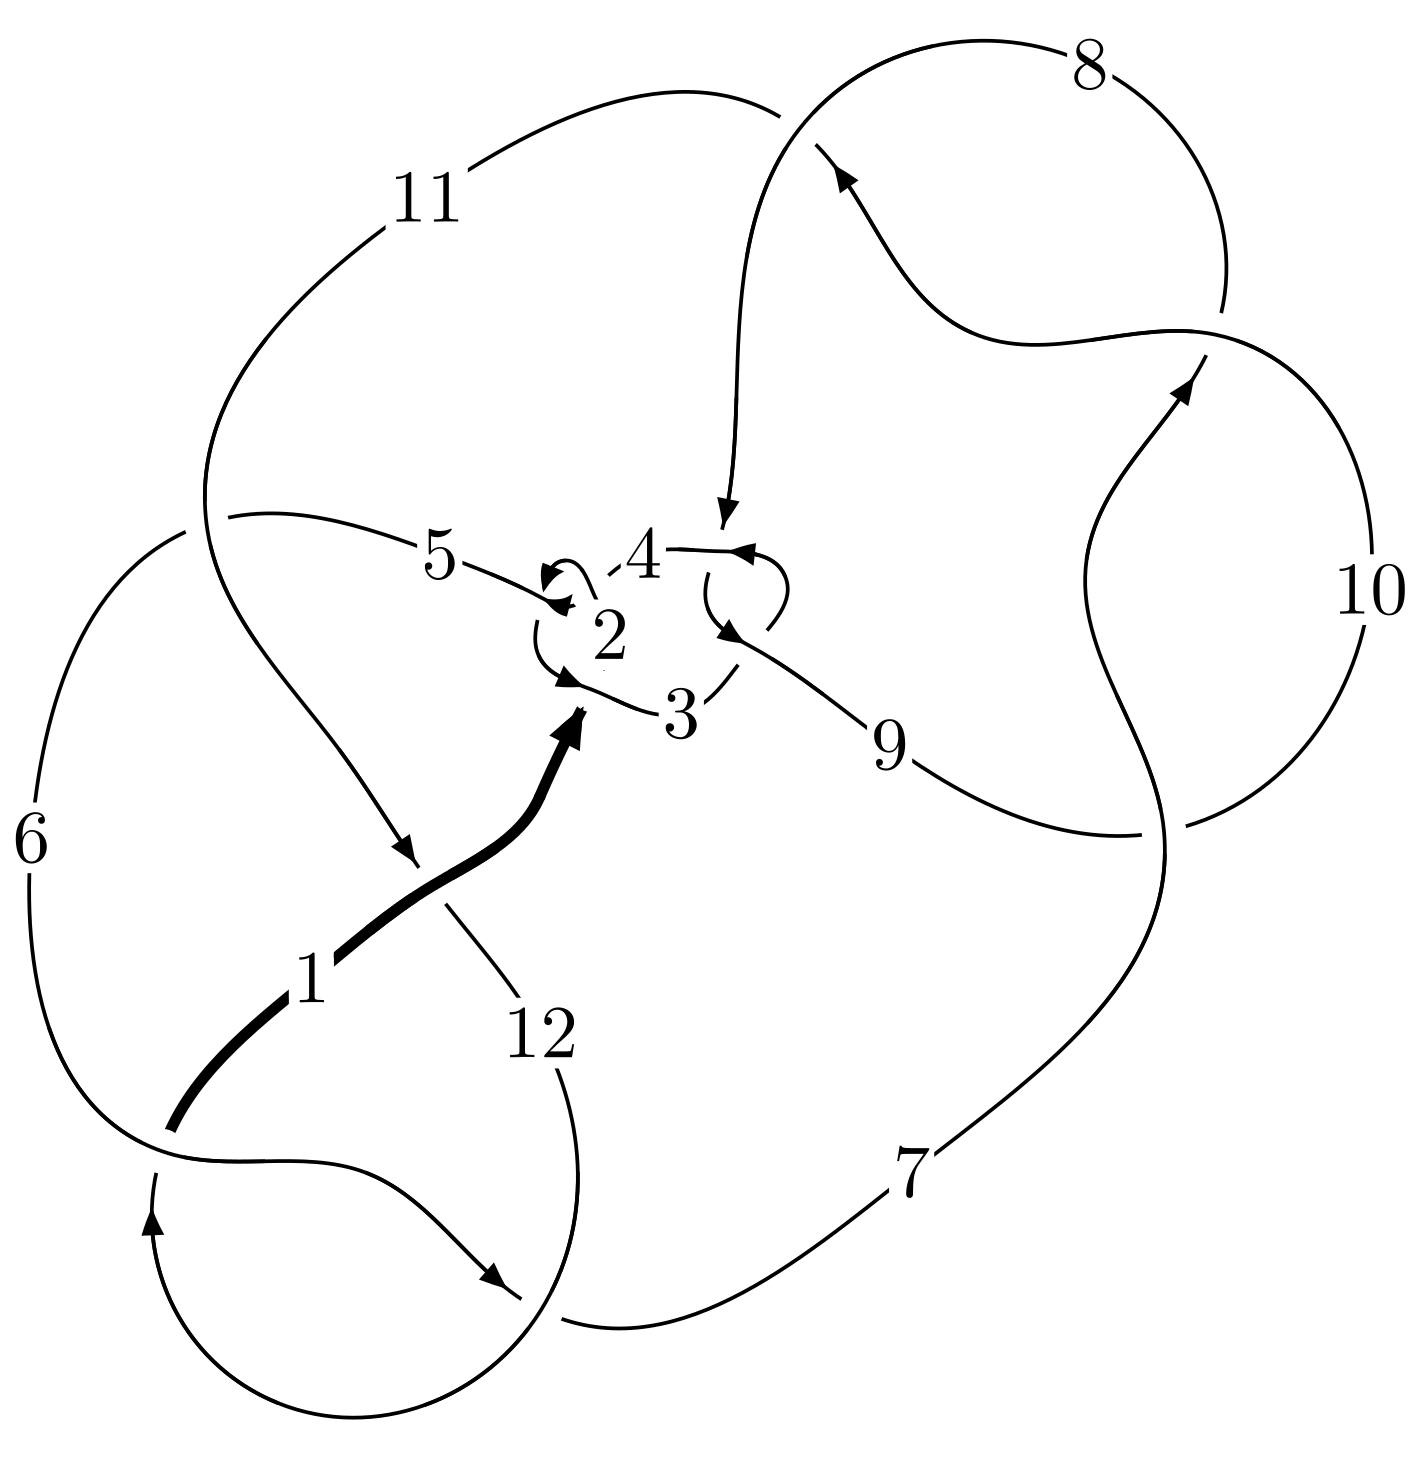
\includegraphics[width=112pt]{../../../GIT/diagram.site/Diagrams/png/958_12a_0157.png}\\
\ \ \ A knot diagram\footnotemark}&
\allowdisplaybreaks
\textbf{Linearized knot diagam} \\
\cline{2-2}
 &
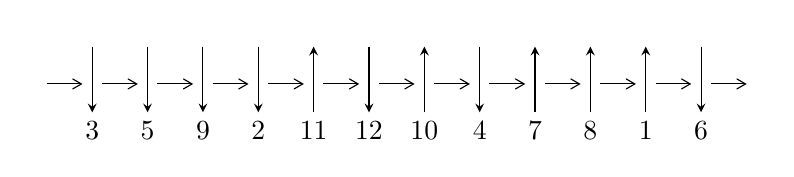
\begin{tikzpicture}[x=20pt, y=17pt]
	% nodes
	\node (C0) at (0, 0) {};
	\node (C1) at (1, 0) {};
	\node (C1U) at (1, +1) {};
	\node (C1D) at (1, -1) {3};

	\node (C2) at (2, 0) {};
	\node (C2U) at (2, +1) {};
	\node (C2D) at (2, -1) {5};

	\node (C3) at (3, 0) {};
	\node (C3U) at (3, +1) {};
	\node (C3D) at (3, -1) {9};

	\node (C4) at (4, 0) {};
	\node (C4U) at (4, +1) {};
	\node (C4D) at (4, -1) {2};

	\node (C5) at (5, 0) {};
	\node (C5U) at (5, +1) {};
	\node (C5D) at (5, -1) {11};

	\node (C6) at (6, 0) {};
	\node (C6U) at (6, +1) {};
	\node (C6D) at (6, -1) {12};

	\node (C7) at (7, 0) {};
	\node (C7U) at (7, +1) {};
	\node (C7D) at (7, -1) {10};

	\node (C8) at (8, 0) {};
	\node (C8U) at (8, +1) {};
	\node (C8D) at (8, -1) {4};

	\node (C9) at (9, 0) {};
	\node (C9U) at (9, +1) {};
	\node (C9D) at (9, -1) {7};

	\node (C10) at (10, 0) {};
	\node (C10U) at (10, +1) {};
	\node (C10D) at (10, -1) {8};

	\node (C11) at (11, 0) {};
	\node (C11U) at (11, +1) {};
	\node (C11D) at (11, -1) {1};

	\node (C12) at (12, 0) {};
	\node (C12U) at (12, +1) {};
	\node (C12D) at (12, -1) {6};
	\node (C13) at (13, 0) {};

	% arrows
	\draw[->,>={angle 60}]
	(C0) edge (C1) (C1) edge (C2) (C2) edge (C3) (C3) edge (C4) (C4) edge (C5) (C5) edge (C6) (C6) edge (C7) (C7) edge (C8) (C8) edge (C9) (C9) edge (C10) (C10) edge (C11) (C11) edge (C12) (C12) edge (C13) ;	\draw[->,>=stealth]
	(C1U) edge (C1D) (C2U) edge (C2D) (C3U) edge (C3D) (C4U) edge (C4D) (C5D) edge (C5U) (C6U) edge (C6D) (C7D) edge (C7U) (C8U) edge (C8D) (C9D) edge (C9U) (C10D) edge (C10U) (C11D) edge (C11U) (C12U) edge (C12D) ;
	\end{tikzpicture} \\
\hhline{~~} \\& 
\textbf{Solving Sequence} \\ \cline{2-2} 
 &
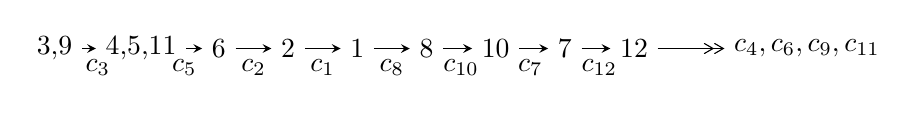
\begin{tikzpicture}[x=25pt, y=7pt]
	% node
	\node (A0) at (-1/8, 0) {3,9};
	\node (A1) at (9/8, 0) {4,5,11};
	\node (A2) at (9/4, 0) {6};
	\node (A3) at (13/4, 0) {2};
	\node (A4) at (17/4, 0) {1};
	\node (A5) at (21/4, 0) {8};
	\node (A6) at (25/4, 0) {10};
	\node (A7) at (29/4, 0) {7};
	\node (A8) at (33/4, 0) {12};
	\node (C1) at (1/2, -1) {$c_{3}$};
	\node (C2) at (7/4, -1) {$c_{5}$};
	\node (C3) at (11/4, -1) {$c_{2}$};
	\node (C4) at (15/4, -1) {$c_{1}$};
	\node (C5) at (19/4, -1) {$c_{8}$};
	\node (C6) at (23/4, -1) {$c_{10}$};
	\node (C7) at (27/4, -1) {$c_{7}$};
	\node (C8) at (31/4, -1) {$c_{12}$};
	\node (A9) at (43/4, 0) {$c_{4},c_{6},c_{9},c_{11}$};

	% edge
	\draw[->,>=stealth]	
	(A0) edge (A1) (A1) edge (A2) (A2) edge (A3) (A3) edge (A4) (A4) edge (A5) (A5) edge (A6) (A6) edge (A7) (A7) edge (A8) ;
	\draw[->>,>={angle 60}]	
	(A8) edge (A9);
\end{tikzpicture} \\ 

\end{tabular} \\

\footnotetext{
The image of knot diagram is generated by the software ``\textbf{Draw programme}" developed by Andrew Bartholomew(\url{http://www.layer8.co.uk/maths/draw/index.htm\#Running-draw}), where we modified some parts for our purpose(\url{https://github.com/CATsTAILs/LinksPainter}).
}\phantom \\ \newline 
\centering \textbf{Ideals for irreducible components\footnotemark of $X_{\text{par}}$} 
 
\begin{align*}
I^u_{1}&=\langle 
-6.07617\times10^{162} u^{76}-1.59683\times10^{163} u^{75}+\cdots+1.45795\times10^{166} d+6.24229\times10^{165},\\
\phantom{I^u_{1}}&\phantom{= \langle  }-7.60333\times10^{161} u^{76}+1.20057\times10^{161} u^{75}+\cdots+3.64487\times10^{165} c+3.09611\times10^{165},\\
\phantom{I^u_{1}}&\phantom{= \langle  }-3.42640\times10^{161} u^{76}+2.87429\times10^{161} u^{75}+\cdots+2.56564\times10^{164} b+1.17150\times10^{165},\\
\phantom{I^u_{1}}&\phantom{= \langle  }6.98505\times10^{162} u^{76}+6.83866\times10^{162} u^{75}+\cdots+1.02626\times10^{165} a-1.03017\times10^{166},\\
\phantom{I^u_{1}}&\phantom{= \langle  }u^{77}+2 u^{76}+\cdots+2560 u^2+512\rangle \\
I^u_{2}&=\langle 
u^3 a^2- a^2 u^2- u^3 a+a^2 u+2 u^3+a u+d-4 a+4,\;u^3 a^2-2 u^3 a+a^2 u+2 u^3+a u+c-2 a+2,\\
\phantom{I^u_{2}}&\phantom{= \langle  }a^2 u^2+b+2 a-2,\;2 u^3 a^2-2 a^2 u^2-3 u^3 a+a^3+2 a^2 u+3 u^2 a+u^3-3 a u- u^2+u,\;u^4+u^2+u+1\rangle \\
I^u_{3}&=\langle 
u^5 a^2-4 u^5 a+2 u^3 a^2+4 u^4 a+4 u^5-5 u^3 a-4 u^4+2 a^2 u+8 u^2 a+6 u^3-3 a u-8 u^2+d+8 a+4 u-8,\\
\phantom{I^u_{3}}&\phantom{= \langle  }-2 u^5 a+u^3 a^2+2 u^4 a+2 u^5-4 u^3 a-2 u^4+a^2 u+4 u^2 a+4 u^3- a u-4 u^2+c+4 a+2 u-4,\\
\phantom{I^u_{3}}&\phantom{= \langle  }a^2 u^2+b+2 a-2,\;-4 u^5 a^2+6 u^5 a+\cdots-6 a+2,\;u^6- u^5+2 u^4-2 u^3+2 u^2-2 u+1\rangle \\
\\
I^v_{1}&=\langle 
c,\;d- v-1,\;b,\;a-1,\;v^2+v+1\rangle \\
I^v_{2}&=\langle 
a,\;d,\;c- v,\;b-1,\;v^2- v+1\rangle \\
I^v_{3}&=\langle 
a,\;d+1,\;c+a,\;b-1,\;v-1\rangle \\
I^v_{4}&=\langle 
a,\;a^2 d- c^2 v-2 c a+c v+a- v,\;d v+1,\;c^2 v^2+2 c a v- v^2 c+a^2- a v+v^2,\;b-1\rangle \\
\end{align*}
\raggedright * 6 irreducible components of $\dim_{\mathbb{C}}=0$, with total 112 representations.\\
\raggedright * 1 irreducible components of $\dim_{\mathbb{C}}=1$ \\
\footnotetext{All coefficients of polynomials are rational numbers. But the coefficients are sometimes approximated in decimal forms when there is not enough margin.}
\newpage
\renewcommand{\arraystretch}{1}
\centering \section*{I. $I^u_{1}= \langle -6.08\times10^{162} u^{76}-1.60\times10^{163} u^{75}+\cdots+1.46\times10^{166} d+6.24\times10^{165},\;-7.60\times10^{161} u^{76}+1.20\times10^{161} u^{75}+\cdots+3.64\times10^{165} c+3.10\times10^{165},\;-3.43\times10^{161} u^{76}+2.87\times10^{161} u^{75}+\cdots+2.57\times10^{164} b+1.17\times10^{165},\;6.99\times10^{162} u^{76}+6.84\times10^{162} u^{75}+\cdots+1.03\times10^{165} a-1.03\times10^{166},\;u^{77}+2 u^{76}+\cdots+2560 u^2+512 \rangle$}
\flushleft \textbf{(i) Arc colorings}\\
\begin{tabular}{m{7pt} m{180pt} m{7pt} m{180pt} }
\flushright $a_{3}=$&$\begin{pmatrix}1\\0\end{pmatrix}$ \\
\flushright $a_{9}=$&$\begin{pmatrix}0\\u\end{pmatrix}$ \\
\flushright $a_{4}=$&$\begin{pmatrix}1\\u^2\end{pmatrix}$ \\
\flushright $a_{5}=$&$\begin{pmatrix}-0.00680634 u^{76}-0.00666370 u^{75}+\cdots-13.3533 u+10.0381\\0.00133550 u^{76}-0.00112030 u^{75}+\cdots+4.56543 u-4.56612\end{pmatrix}$ \\
\flushright $a_{11}=$&$\begin{pmatrix}0.000208604 u^{76}-0.0000329385 u^{75}+\cdots-1.00214 u-0.849444\\0.000416762 u^{76}+0.00109526 u^{75}+\cdots+0.259754 u-0.428156\end{pmatrix}$ \\
\flushright $a_{6}=$&$\begin{pmatrix}-0.00584350 u^{76}-0.00606296 u^{75}+\cdots-10.5775 u+9.19500\\-0.000891648 u^{76}-0.00576153 u^{75}+\cdots+4.16493 u-3.32748\end{pmatrix}$ \\
\flushright $a_{2}=$&$\begin{pmatrix}-0.00680634 u^{76}-0.00666370 u^{75}+\cdots-13.3533 u+10.0381\\0.000152722 u^{76}+0.00152555 u^{75}+\cdots-1.08059 u+1.00825\end{pmatrix}$ \\
\flushright $a_{1}=$&$\begin{pmatrix}-0.00665361 u^{76}-0.00513815 u^{75}+\cdots-14.4339 u+11.0464\\0.000152722 u^{76}+0.00152555 u^{75}+\cdots-1.08059 u+1.00825\end{pmatrix}$ \\
\flushright $a_{8}=$&$\begin{pmatrix}u\\u^3+u\end{pmatrix}$ \\
\flushright $a_{10}=$&$\begin{pmatrix}-0.0000869789 u^{76}-0.000560439 u^{75}+\cdots-0.853173 u-0.579783\\0.000218526 u^{76}+0.000662503 u^{75}+\cdots+0.560059 u-0.191092\end{pmatrix}$ \\
\flushright $a_{7}=$&$\begin{pmatrix}0.000290951 u^{76}+0.00110858 u^{75}+\cdots+1.36870 u+0.190813\\0.000499554 u^{76}+0.00107564 u^{75}+\cdots+0.366559 u-0.658630\end{pmatrix}$ \\
\flushright $a_{12}=$&$\begin{pmatrix}0.00628963 u^{76}+0.0183729 u^{75}+\cdots+6.15552 u+8.93643\\-0.00429774 u^{76}-0.00774981 u^{75}+\cdots-6.38490 u-0.700057\end{pmatrix}$\\&\end{tabular}
\flushleft \textbf{(ii) Obstruction class $= -1$}\\~\\
\flushleft \textbf{(iii) Cusp Shapes $= -0.0221138 u^{76}-0.0478032 u^{75}+\cdots-21.6023 u+0.388088$}\\~\\
\newpage\renewcommand{\arraystretch}{1}
\flushleft \textbf{(iv) u-Polynomials at the component}\newline \\
\begin{tabular}{m{50pt}|m{274pt}}
Crossings & \hspace{64pt}u-Polynomials at each crossing \\
\hline $$\begin{aligned}c_{1}\end{aligned}$$&$\begin{aligned}
&u^{77}+34 u^{76}+\cdots+1568 u+256
\end{aligned}$\\
\hline $$\begin{aligned}c_{2},c_{4}\end{aligned}$$&$\begin{aligned}
&u^{77}-8 u^{76}+\cdots-72 u+16
\end{aligned}$\\
\hline $$\begin{aligned}c_{3},c_{8}\end{aligned}$$&$\begin{aligned}
&u^{77}+2 u^{76}+\cdots+2560 u^2+512
\end{aligned}$\\
\hline $$\begin{aligned}c_{5}\end{aligned}$$&$\begin{aligned}
&u^{77}+2 u^{76}+\cdots+351912 u+66564
\end{aligned}$\\
\hline $$\begin{aligned}c_{6},c_{12}\end{aligned}$$&$\begin{aligned}
&u^{77}-2 u^{76}+\cdots-27 u^2+4
\end{aligned}$\\
\hline $$\begin{aligned}c_{7},c_{9},c_{10}\end{aligned}$$&$\begin{aligned}
&u^{77}+8 u^{76}+\cdots-72 u+16
\end{aligned}$\\
\hline $$\begin{aligned}c_{11}\end{aligned}$$&$\begin{aligned}
&u^{77}-36 u^{76}+\cdots+216 u+16
\end{aligned}$\\
\hline
\end{tabular}\\~\\
\newpage\renewcommand{\arraystretch}{1}
\flushleft \textbf{(v) Riley Polynomials at the component}\newline \\
\begin{tabular}{m{50pt}|m{274pt}}
Crossings & \hspace{64pt}Riley Polynomials at each crossing \\
\hline $$\begin{aligned}c_{1}\end{aligned}$$&$\begin{aligned}
&y^{77}+26 y^{76}+\cdots+3416576 y-65536
\end{aligned}$\\
\hline $$\begin{aligned}c_{2},c_{4}\end{aligned}$$&$\begin{aligned}
&y^{77}-34 y^{76}+\cdots+1568 y-256
\end{aligned}$\\
\hline $$\begin{aligned}c_{3},c_{8}\end{aligned}$$&$\begin{aligned}
&y^{77}+30 y^{76}+\cdots-2621440 y-262144
\end{aligned}$\\
\hline $$\begin{aligned}c_{5}\end{aligned}$$&$\begin{aligned}
&y^{77}-12 y^{76}+\cdots+120020616504 y-4430766096
\end{aligned}$\\
\hline $$\begin{aligned}c_{6},c_{12}\end{aligned}$$&$\begin{aligned}
&y^{77}+36 y^{76}+\cdots+216 y-16
\end{aligned}$\\
\hline $$\begin{aligned}c_{7},c_{9},c_{10}\end{aligned}$$&$\begin{aligned}
&y^{77}-74 y^{76}+\cdots+7712 y-256
\end{aligned}$\\
\hline $$\begin{aligned}c_{11}\end{aligned}$$&$\begin{aligned}
&y^{77}+12 y^{76}+\cdots+84256 y-256
\end{aligned}$\\
\hline
\end{tabular}\\~\\
\newpage\flushleft \textbf{(vi) Complex Volumes and Cusp Shapes}
$$\begin{array}{c|c|c}  
\text{Solutions to }I^u_{1}& \I (\text{vol} + \sqrt{-1}CS) & \text{Cusp shape}\\
 \hline 
\begin{aligned}
u &= -0.508886 + 0.845592 I \\
a &= \phantom{-}0.440978 - 0.047456 I \\
b &= \phantom{-}1.241720 + 0.241243 I \\
c &= \phantom{-}1.093870 + 0.364160 I \\
d &= \phantom{-}0.443416 - 0.224335 I\end{aligned}
 & -2.40889 + 4.27390 I & -3.74115 - 6.44221 I \\ \hline\begin{aligned}
u &= -0.508886 - 0.845592 I \\
a &= \phantom{-}0.440978 + 0.047456 I \\
b &= \phantom{-}1.241720 - 0.241243 I \\
c &= \phantom{-}1.093870 - 0.364160 I \\
d &= \phantom{-}0.443416 + 0.224335 I\end{aligned}
 & -2.40889 - 4.27390 I & -3.74115 + 6.44221 I \\ \hline\begin{aligned}
u &= \phantom{-}0.848496 + 0.585068 I \\
a &= \phantom{-}0.460618 + 0.092632 I \\
b &= \phantom{-}1.086610 - 0.419625 I \\
c &= -0.531801 + 1.113610 I \\
d &= -1.32944 + 1.48023 I\end{aligned}
 & -3.78378 + 2.11500 I & -7.65464 - 1.99007 I \\ \hline\begin{aligned}
u &= \phantom{-}0.848496 - 0.585068 I \\
a &= \phantom{-}0.460618 - 0.092632 I \\
b &= \phantom{-}1.086610 + 0.419625 I \\
c &= -0.531801 - 1.113610 I \\
d &= -1.32944 - 1.48023 I\end{aligned}
 & -3.78378 - 2.11500 I & -7.65464 + 1.99007 I \\ \hline\begin{aligned}
u &= \phantom{-}0.990280 + 0.319237 I \\
a &= \phantom{-}0.580990 - 0.275212 I \\
b &= \phantom{-}0.405766 + 0.665904 I \\
c &= \phantom{-}0.427768 - 0.711040 I \\
d &= \phantom{-}0.003575 - 0.815149 I\end{aligned}
 & \phantom{-}2.98745 + 0.86657 I & \phantom{-0.000000 } 0 \\ \hline\begin{aligned}
u &= \phantom{-}0.990280 - 0.319237 I \\
a &= \phantom{-}0.580990 + 0.275212 I \\
b &= \phantom{-}0.405766 - 0.665904 I \\
c &= \phantom{-}0.427768 + 0.711040 I \\
d &= \phantom{-}0.003575 + 0.815149 I\end{aligned}
 & \phantom{-}2.98745 - 0.86657 I & \phantom{-0.000000 } 0\\
 \hline 
 \end{array}$$\newpage$$\begin{array}{c|c|c}  
\text{Solutions to }I^u_{1}& \I (\text{vol} + \sqrt{-1}CS) & \text{Cusp shape}\\
 \hline 
\begin{aligned}
u &= \phantom{-}0.617221 + 0.733532 I \\
a &= \phantom{-}0.450662 + 0.060640 I \\
b &= \phantom{-}1.179500 - 0.293267 I \\
c &= -0.865693 + 0.615479 I \\
d &= -0.818586 + 0.224399 I\end{aligned}
 & -4.09446 + 0.35704 I & -8.04104 + 0.70386 I \\ \hline\begin{aligned}
u &= \phantom{-}0.617221 - 0.733532 I \\
a &= \phantom{-}0.450662 - 0.060640 I \\
b &= \phantom{-}1.179500 + 0.293267 I \\
c &= -0.865693 - 0.615479 I \\
d &= -0.818586 - 0.224399 I\end{aligned}
 & -4.09446 - 0.35704 I & -8.04104 - 0.70386 I \\ \hline\begin{aligned}
u &= -0.517431 + 0.792256 I \\
a &= -0.31513 - 2.57319 I \\
b &= -1.046890 + 0.382880 I \\
c &= \phantom{-}0.979361 + 0.392885 I \\
d &= \phantom{-}0.491329 - 0.041258 I\end{aligned}
 & -2.57405 - 0.08416 I & -4.54592 - 2.74373 I \\ \hline\begin{aligned}
u &= -0.517431 - 0.792256 I \\
a &= -0.31513 + 2.57319 I \\
b &= -1.046890 - 0.382880 I \\
c &= \phantom{-}0.979361 - 0.392885 I \\
d &= \phantom{-}0.491329 + 0.041258 I\end{aligned}
 & -2.57405 + 0.08416 I & -4.54592 + 2.74373 I \\ \hline\begin{aligned}
u &= \phantom{-}0.082487 + 0.936352 I \\
a &= \phantom{-}0.92003 - 1.14713 I \\
b &= -0.574527 + 0.530498 I \\
c &= \phantom{-}1.17847 - 0.94179 I \\
d &= -0.290045 + 0.776854 I\end{aligned}
 & \phantom{-}1.72016 + 1.41215 I & \phantom{-}1.65188 - 3.77223 I \\ \hline\begin{aligned}
u &= \phantom{-}0.082487 - 0.936352 I \\
a &= \phantom{-}0.92003 + 1.14713 I \\
b &= -0.574527 - 0.530498 I \\
c &= \phantom{-}1.17847 + 0.94179 I \\
d &= -0.290045 - 0.776854 I\end{aligned}
 & \phantom{-}1.72016 - 1.41215 I & \phantom{-}1.65188 + 3.77223 I\\
 \hline 
 \end{array}$$\newpage$$\begin{array}{c|c|c}  
\text{Solutions to }I^u_{1}& \I (\text{vol} + \sqrt{-1}CS) & \text{Cusp shape}\\
 \hline 
\begin{aligned}
u &= \phantom{-}0.582500 + 0.889546 I \\
a &= -0.41276 + 2.17080 I \\
b &= -1.084530 - 0.444586 I \\
c &= -1.204890 + 0.519522 I \\
d &= -0.720160 - 0.450817 I\end{aligned}
 & -3.62010 - 5.07823 I & -6.10660 + 7.37918 I \\ \hline\begin{aligned}
u &= \phantom{-}0.582500 - 0.889546 I \\
a &= -0.41276 - 2.17080 I \\
b &= -1.084530 + 0.444586 I \\
c &= -1.204890 - 0.519522 I \\
d &= -0.720160 + 0.450817 I\end{aligned}
 & -3.62010 + 5.07823 I & -6.10660 - 7.37918 I \\ \hline\begin{aligned}
u &= -0.228301 + 1.040040 I \\
a &= \phantom{-}0.723676 + 0.951160 I \\
b &= -0.493370 - 0.665886 I \\
c &= -0.513216 - 0.329220 I \\
d &= -0.312338 - 0.999680 I\end{aligned}
 & \phantom{-}3.92825 - 1.69884 I & \phantom{-}4.65730 + 2.32962 I \\ \hline\begin{aligned}
u &= -0.228301 - 1.040040 I \\
a &= \phantom{-}0.723676 - 0.951160 I \\
b &= -0.493370 + 0.665886 I \\
c &= -0.513216 + 0.329220 I \\
d &= -0.312338 + 0.999680 I\end{aligned}
 & \phantom{-}3.92825 + 1.69884 I & \phantom{-}4.65730 - 2.32962 I \\ \hline\begin{aligned}
u &= -0.782003 + 0.468875 I \\
a &= \phantom{-}0.479369 - 0.088840 I \\
b &= \phantom{-}1.016810 + 0.373767 I \\
c &= -0.789013 - 1.040910 I \\
d &= -0.598791 - 0.392671 I\end{aligned}
 & -0.65497 - 3.51390 I & -3.54011 + 4.44478 I \\ \hline\begin{aligned}
u &= -0.782003 - 0.468875 I \\
a &= \phantom{-}0.479369 + 0.088840 I \\
b &= \phantom{-}1.016810 - 0.373767 I \\
c &= -0.789013 + 1.040910 I \\
d &= -0.598791 + 0.392671 I\end{aligned}
 & -0.65497 + 3.51390 I & -3.54011 - 4.44478 I\\
 \hline 
 \end{array}$$\newpage$$\begin{array}{c|c|c}  
\text{Solutions to }I^u_{1}& \I (\text{vol} + \sqrt{-1}CS) & \text{Cusp shape}\\
 \hline 
\begin{aligned}
u &= \phantom{-}0.374962 + 1.039940 I \\
a &= \phantom{-}0.679703 - 0.804881 I \\
b &= -0.387561 + 0.725229 I \\
c &= \phantom{-}0.822403 - 0.322418 I \\
d &= \phantom{-}0.559284 - 0.573519 I\end{aligned}
 & \phantom{-}3.38837 - 3.78470 I & \phantom{-0.000000 } 0 \\ \hline\begin{aligned}
u &= \phantom{-}0.374962 - 1.039940 I \\
a &= \phantom{-}0.679703 + 0.804881 I \\
b &= -0.387561 - 0.725229 I \\
c &= \phantom{-}0.822403 + 0.322418 I \\
d &= \phantom{-}0.559284 + 0.573519 I\end{aligned}
 & \phantom{-}3.38837 + 3.78470 I & \phantom{-0.000000 } 0 \\ \hline\begin{aligned}
u &= -0.965284 + 0.548957 I \\
a &= \phantom{-}0.458449 - 0.109175 I \\
b &= \phantom{-}1.064210 + 0.491568 I \\
c &= \phantom{-}0.42927 + 1.36968 I \\
d &= \phantom{-}1.62931 + 2.26420 I\end{aligned}
 & -1.81197 - 6.85619 I & \phantom{-0.000000 } 0 \\ \hline\begin{aligned}
u &= -0.965284 - 0.548957 I \\
a &= \phantom{-}0.458449 + 0.109175 I \\
b &= \phantom{-}1.064210 - 0.491568 I \\
c &= \phantom{-}0.42927 - 1.36968 I \\
d &= \phantom{-}1.62931 - 2.26420 I\end{aligned}
 & -1.81197 + 6.85619 I & \phantom{-0.000000 } 0 \\ \hline\begin{aligned}
u &= -0.288832 + 1.092220 I \\
a &= \phantom{-}0.655250 + 0.897222 I \\
b &= -0.469158 - 0.726873 I \\
c &= -1.39360 - 1.30383 I \\
d &= \phantom{-}0.03743 + 1.65696 I\end{aligned}
 & \phantom{-}4.40655 + 2.61636 I & \phantom{-0.000000 } 0 \\ \hline\begin{aligned}
u &= -0.288832 - 1.092220 I \\
a &= \phantom{-}0.655250 - 0.897222 I \\
b &= -0.469158 + 0.726873 I \\
c &= -1.39360 + 1.30383 I \\
d &= \phantom{-}0.03743 - 1.65696 I\end{aligned}
 & \phantom{-}4.40655 - 2.61636 I & \phantom{-0.000000 } 0\\
 \hline 
 \end{array}$$\newpage$$\begin{array}{c|c|c}  
\text{Solutions to }I^u_{1}& \I (\text{vol} + \sqrt{-1}CS) & \text{Cusp shape}\\
 \hline 
\begin{aligned}
u &= -0.815552 + 0.276755 I \\
a &= \phantom{-}0.510621 - 0.104384 I \\
b &= \phantom{-}0.879842 + 0.384286 I \\
c &= -0.134802 + 0.964627 I \\
d &= -0.35977 + 2.02275 I\end{aligned}
 & \phantom{-}0.065597 - 0.205341 I & -1.21551 + 1.86968 I \\ \hline\begin{aligned}
u &= -0.815552 - 0.276755 I \\
a &= \phantom{-}0.510621 + 0.104384 I \\
b &= \phantom{-}0.879842 - 0.384286 I \\
c &= -0.134802 - 0.964627 I \\
d &= -0.35977 - 2.02275 I\end{aligned}
 & \phantom{-}0.065597 + 0.205341 I & -1.21551 - 1.86968 I \\ \hline\begin{aligned}
u &= \phantom{-}0.008067 + 1.164640 I \\
a &= \phantom{-}0.524425 + 1.231070 I \\
b &= -0.707115 - 0.687536 I \\
c &= -1.63638 - 0.81487 I \\
d &= \phantom{-}1.18786 + 0.86080 I\end{aligned}
 & \phantom{-}4.97078 - 4.99360 I & \phantom{-0.000000 } 0 \\ \hline\begin{aligned}
u &= \phantom{-}0.008067 - 1.164640 I \\
a &= \phantom{-}0.524425 - 1.231070 I \\
b &= -0.707115 + 0.687536 I \\
c &= -1.63638 + 0.81487 I \\
d &= \phantom{-}1.18786 - 0.86080 I\end{aligned}
 & \phantom{-}4.97078 + 4.99360 I & \phantom{-0.000000 } 0 \\ \hline\begin{aligned}
u &= -1.177360 + 0.140655 I \\
a &= \phantom{-}0.514925 + 0.236545 I \\
b &= \phantom{-}0.603622 - 0.736667 I \\
c &= -0.027412 - 0.316988 I \\
d &= \phantom{-}1.016250 - 0.656214 I\end{aligned}
 & \phantom{-}6.72367 + 2.38646 I & \phantom{-0.000000 } 0 \\ \hline\begin{aligned}
u &= -1.177360 - 0.140655 I \\
a &= \phantom{-}0.514925 - 0.236545 I \\
b &= \phantom{-}0.603622 + 0.736667 I \\
c &= -0.027412 + 0.316988 I \\
d &= \phantom{-}1.016250 + 0.656214 I\end{aligned}
 & \phantom{-}6.72367 - 2.38646 I & \phantom{-0.000000 } 0\\
 \hline 
 \end{array}$$\newpage$$\begin{array}{c|c|c}  
\text{Solutions to }I^u_{1}& \I (\text{vol} + \sqrt{-1}CS) & \text{Cusp shape}\\
 \hline 
\begin{aligned}
u &= \phantom{-}0.516220 + 1.088150 I \\
a &= -0.14742 + 1.74242 I \\
b &= -1.048210 - 0.569836 I \\
c &= \phantom{-}1.105030 - 0.234332 I \\
d &= \phantom{-}0.652838 + 0.110822 I\end{aligned}
 & \phantom{-}2.28765 - 3.11487 I & \phantom{-0.000000 } 0 \\ \hline\begin{aligned}
u &= \phantom{-}0.516220 - 1.088150 I \\
a &= -0.14742 - 1.74242 I \\
b &= -1.048210 + 0.569836 I \\
c &= \phantom{-}1.105030 + 0.234332 I \\
d &= \phantom{-}0.652838 - 0.110822 I\end{aligned}
 & \phantom{-}2.28765 + 3.11487 I & \phantom{-0.000000 } 0 \\ \hline\begin{aligned}
u &= -1.143240 + 0.423905 I \\
a &= \phantom{-}0.533939 + 0.311288 I \\
b &= \phantom{-}0.397778 - 0.814910 I \\
c &= -0.113421 - 0.926777 I \\
d &= -0.01193 - 1.62150 I\end{aligned}
 & \phantom{-}5.54743 - 5.38085 I & \phantom{-0.000000 } 0 \\ \hline\begin{aligned}
u &= -1.143240 - 0.423905 I \\
a &= \phantom{-}0.533939 - 0.311288 I \\
b &= \phantom{-}0.397778 + 0.814910 I \\
c &= -0.113421 + 0.926777 I \\
d &= -0.01193 + 1.62150 I\end{aligned}
 & \phantom{-}5.54743 + 5.38085 I & \phantom{-0.000000 } 0 \\ \hline\begin{aligned}
u &= -1.079500 + 0.575143 I \\
a &= \phantom{-}0.447329 - 0.120477 I \\
b &= \phantom{-}1.084300 + 0.561354 I \\
c &= -0.260355 - 1.216300 I \\
d &= -0.90050 - 1.58646 I\end{aligned}
 & \phantom{-}1.00971 - 5.65602 I & \phantom{-0.000000 } 0 \\ \hline\begin{aligned}
u &= -1.079500 - 0.575143 I \\
a &= \phantom{-}0.447329 + 0.120477 I \\
b &= \phantom{-}1.084300 - 0.561354 I \\
c &= -0.260355 + 1.216300 I \\
d &= -0.90050 + 1.58646 I\end{aligned}
 & \phantom{-}1.00971 + 5.65602 I & \phantom{-0.000000 } 0\\
 \hline 
 \end{array}$$\newpage$$\begin{array}{c|c|c}  
\text{Solutions to }I^u_{1}& \I (\text{vol} + \sqrt{-1}CS) & \text{Cusp shape}\\
 \hline 
\begin{aligned}
u &= \phantom{-}1.163010 + 0.411297 I \\
a &= \phantom{-}0.457972 + 0.144139 I \\
b &= \phantom{-}0.986739 - 0.625293 I \\
c &= \phantom{-}0.071233 - 0.902749 I \\
d &= -0.10463 - 1.67523 I\end{aligned}
 & \phantom{-}5.58247 + 2.79509 I & \phantom{-0.000000 } 0 \\ \hline\begin{aligned}
u &= \phantom{-}1.163010 - 0.411297 I \\
a &= \phantom{-}0.457972 - 0.144139 I \\
b &= \phantom{-}0.986739 + 0.625293 I \\
c &= \phantom{-}0.071233 + 0.902749 I \\
d &= -0.10463 + 1.67523 I\end{aligned}
 & \phantom{-}5.58247 - 2.79509 I & \phantom{-0.000000 } 0 \\ \hline\begin{aligned}
u &= -0.530613 + 1.137340 I \\
a &= -0.16592 - 1.65105 I \\
b &= -1.060260 + 0.599620 I \\
c &= \phantom{-}1.76242 + 0.34399 I \\
d &= -0.11353 - 1.60654 I\end{aligned}
 & \phantom{-}2.68982 + 5.10175 I & \phantom{-0.000000 } 0 \\ \hline\begin{aligned}
u &= -0.530613 - 1.137340 I \\
a &= -0.16592 + 1.65105 I \\
b &= -1.060260 - 0.599620 I \\
c &= \phantom{-}1.76242 - 0.34399 I \\
d &= -0.11353 + 1.60654 I\end{aligned}
 & \phantom{-}2.68982 - 5.10175 I & \phantom{-0.000000 } 0 \\ \hline\begin{aligned}
u &= -0.601554 + 1.104580 I \\
a &= -0.29797 - 1.68572 I \\
b &= -1.101680 + 0.575244 I \\
c &= -1.271520 - 0.218579 I \\
d &= -0.788648 + 0.590297 I\end{aligned}
 & \phantom{-}1.29562 + 8.75795 I & \phantom{-0.000000 } 0 \\ \hline\begin{aligned}
u &= -0.601554 - 1.104580 I \\
a &= -0.29797 + 1.68572 I \\
b &= -1.101680 - 0.575244 I \\
c &= -1.271520 + 0.218579 I \\
d &= -0.788648 - 0.590297 I\end{aligned}
 & \phantom{-}1.29562 - 8.75795 I & \phantom{-0.000000 } 0\\
 \hline 
 \end{array}$$\newpage$$\begin{array}{c|c|c}  
\text{Solutions to }I^u_{1}& \I (\text{vol} + \sqrt{-1}CS) & \text{Cusp shape}\\
 \hline 
\begin{aligned}
u &= \phantom{-}0.666542 + 1.084300 I \\
a &= -0.41901 + 1.68178 I \\
b &= -1.139490 - 0.559856 I \\
c &= -1.67095 + 0.67803 I \\
d &= -0.92819 - 1.72084 I\end{aligned}
 & -2.21245 - 7.79054 I & \phantom{-0.000000 } 0 \\ \hline\begin{aligned}
u &= \phantom{-}0.666542 - 1.084300 I \\
a &= -0.41901 - 1.68178 I \\
b &= -1.139490 + 0.559856 I \\
c &= -1.67095 - 0.67803 I \\
d &= -0.92819 + 1.72084 I\end{aligned}
 & -2.21245 + 7.79054 I & \phantom{-0.000000 } 0 \\ \hline\begin{aligned}
u &= \phantom{-}0.620529 + 0.325559 I \\
a &= \phantom{-}0.505847 + 0.065088 I \\
b &= \phantom{-}0.944687 - 0.250227 I \\
c &= \phantom{-}1.17082 - 0.90601 I \\
d &= \phantom{-}0.328371 - 0.105641 I\end{aligned}
 & \phantom{-}0.115678 - 1.341920 I & -2.41782 + 1.83708 I \\ \hline\begin{aligned}
u &= \phantom{-}0.620529 - 0.325559 I \\
a &= \phantom{-}0.505847 - 0.065088 I \\
b &= \phantom{-}0.944687 + 0.250227 I \\
c &= \phantom{-}1.17082 + 0.90601 I \\
d &= \phantom{-}0.328371 + 0.105641 I\end{aligned}
 & \phantom{-}0.115678 + 1.341920 I & -2.41782 - 1.83708 I \\ \hline\begin{aligned}
u &= \phantom{-}1.161000 + 0.625559 I \\
a &= \phantom{-}0.435979 + 0.124995 I \\
b &= \phantom{-}1.119470 - 0.607651 I \\
c &= \phantom{-}0.116799 - 1.332580 I \\
d &= \phantom{-}1.12055 - 2.13672 I\end{aligned}
 & \phantom{-}3.39852 + 10.69180 I & \phantom{-0.000000 } 0 \\ \hline\begin{aligned}
u &= \phantom{-}1.161000 - 0.625559 I \\
a &= \phantom{-}0.435979 - 0.124995 I \\
b &= \phantom{-}1.119470 + 0.607651 I \\
c &= \phantom{-}0.116799 + 1.332580 I \\
d &= \phantom{-}1.12055 + 2.13672 I\end{aligned}
 & \phantom{-}3.39852 - 10.69180 I & \phantom{-0.000000 } 0\\
 \hline 
 \end{array}$$\newpage$$\begin{array}{c|c|c}  
\text{Solutions to }I^u_{1}& \I (\text{vol} + \sqrt{-1}CS) & \text{Cusp shape}\\
 \hline 
\begin{aligned}
u &= \phantom{-}0.423653 + 0.527399 I \\
a &= \phantom{-}0.911492 - 0.383290 I \\
b &= -0.067745 + 0.392021 I \\
c &= \phantom{-}1.10825 - 1.37074 I \\
d &= \phantom{-}0.418849 + 0.237150 I\end{aligned}
 & \phantom{-}1.92120 + 0.81846 I & \phantom{-}4.58107 + 0.87681 I \\ \hline\begin{aligned}
u &= \phantom{-}0.423653 - 0.527399 I \\
a &= \phantom{-}0.911492 + 0.383290 I \\
b &= -0.067745 - 0.392021 I \\
c &= \phantom{-}1.10825 + 1.37074 I \\
d &= \phantom{-}0.418849 - 0.237150 I\end{aligned}
 & \phantom{-}1.92120 - 0.81846 I & \phantom{-}4.58107 - 0.87681 I \\ \hline\begin{aligned}
u &= \phantom{-}0.662834 + 0.003253 I \\
a &= \phantom{-}0.620162 + 0.068360 I \\
b &= \phantom{-}0.593125 - 0.175609 I \\
c &= \phantom{-}0.844082 + 0.426336 I \\
d &= \phantom{-}2.08843 + 0.88000 I\end{aligned}
 & \phantom{-}0.58945 + 2.77011 I & -1.22579 - 6.61866 I \\ \hline\begin{aligned}
u &= \phantom{-}0.662834 - 0.003253 I \\
a &= \phantom{-}0.620162 - 0.068360 I \\
b &= \phantom{-}0.593125 + 0.175609 I \\
c &= \phantom{-}0.844082 - 0.426336 I \\
d &= \phantom{-}2.08843 - 0.88000 I\end{aligned}
 & \phantom{-}0.58945 - 2.77011 I & -1.22579 + 6.61866 I \\ \hline\begin{aligned}
u &= -0.703559 + 1.143570 I \\
a &= -0.43434 - 1.56703 I \\
b &= -1.164260 + 0.592620 I \\
c &= \phantom{-}1.82114 + 0.75444 I \\
d &= \phantom{-}1.05029 - 2.27985 I\end{aligned}
 & \phantom{-}0.07596 + 12.98220 I & \phantom{-0.000000 } 0 \\ \hline\begin{aligned}
u &= -0.703559 - 1.143570 I \\
a &= -0.43434 + 1.56703 I \\
b &= -1.164260 - 0.592620 I \\
c &= \phantom{-}1.82114 - 0.75444 I \\
d &= \phantom{-}1.05029 + 2.27985 I\end{aligned}
 & \phantom{-}0.07596 - 12.98220 I & \phantom{-0.000000 } 0\\
 \hline 
 \end{array}$$\newpage$$\begin{array}{c|c|c}  
\text{Solutions to }I^u_{1}& \I (\text{vol} + \sqrt{-1}CS) & \text{Cusp shape}\\
 \hline 
\begin{aligned}
u &= \phantom{-}0.624723 + 1.201920 I \\
a &= \phantom{-}0.513586 - 0.684350 I \\
b &= -0.298481 + 0.934769 I \\
c &= \phantom{-}1.343470 - 0.036213 I \\
d &= \phantom{-}0.266666 + 0.986054 I\end{aligned}
 & \phantom{-}5.70918 - 6.67323 I & \phantom{-0.000000 } 0 \\ \hline\begin{aligned}
u &= \phantom{-}0.624723 - 1.201920 I \\
a &= \phantom{-}0.513586 + 0.684350 I \\
b &= -0.298481 - 0.934769 I \\
c &= \phantom{-}1.343470 + 0.036213 I \\
d &= \phantom{-}0.266666 - 0.986054 I\end{aligned}
 & \phantom{-}5.70918 + 6.67323 I & \phantom{-0.000000 } 0 \\ \hline\begin{aligned}
u &= -0.127875 + 0.624992 I \\
a &= \phantom{-}0.463873 - 0.011490 I \\
b &= \phantom{-}1.154440 + 0.053363 I \\
c &= \phantom{-}0.435762 - 0.358619 I \\
d &= -0.038269 + 0.332638 I\end{aligned}
 & -0.93270 - 1.56780 I & \phantom{-}1.99036 - 0.81001 I \\ \hline\begin{aligned}
u &= -0.127875 - 0.624992 I \\
a &= \phantom{-}0.463873 + 0.011490 I \\
b &= \phantom{-}1.154440 - 0.053363 I \\
c &= \phantom{-}0.435762 + 0.358619 I \\
d &= -0.038269 - 0.332638 I\end{aligned}
 & -0.93270 + 1.56780 I & \phantom{-}1.99036 + 0.81001 I \\ \hline\begin{aligned}
u &= \phantom{-}0.115044 + 1.357830 I \\
a &= \phantom{-}0.267455 + 1.195870 I \\
b &= -0.821892 - 0.796376 I \\
c &= \phantom{-}0.264755 + 0.381750 I \\
d &= -0.286633 - 1.330580 I\end{aligned}
 & \phantom{-}9.14335 - 2.92995 I & \phantom{-0.000000 } 0 \\ \hline\begin{aligned}
u &= \phantom{-}0.115044 - 1.357830 I \\
a &= \phantom{-}0.267455 - 1.195870 I \\
b &= -0.821892 + 0.796376 I \\
c &= \phantom{-}0.264755 - 0.381750 I \\
d &= -0.286633 + 1.330580 I\end{aligned}
 & \phantom{-}9.14335 + 2.92995 I & \phantom{-0.000000 } 0\\
 \hline 
 \end{array}$$\newpage$$\begin{array}{c|c|c}  
\text{Solutions to }I^u_{1}& \I (\text{vol} + \sqrt{-1}CS) & \text{Cusp shape}\\
 \hline 
\begin{aligned}
u &= -0.518606 + 1.307430 I \\
a &= \phantom{-}0.471054 + 0.753719 I \\
b &= -0.403718 - 0.954094 I \\
c &= -1.155440 + 0.212036 I \\
d &= \phantom{-}0.575561 + 0.435533 I\end{aligned}
 & \phantom{-}10.68990 + 3.50430 I & \phantom{-0.000000 } 0 \\ \hline\begin{aligned}
u &= -0.518606 - 1.307430 I \\
a &= \phantom{-}0.471054 - 0.753719 I \\
b &= -0.403718 + 0.954094 I \\
c &= -1.155440 - 0.212036 I \\
d &= \phantom{-}0.575561 - 0.435533 I\end{aligned}
 & \phantom{-}10.68990 - 3.50430 I & \phantom{-0.000000 } 0 \\ \hline\begin{aligned}
u &= -0.758435 + 1.184640 I \\
a &= -0.47779 - 1.47703 I \\
b &= -1.198260 + 0.612902 I \\
c &= -1.59692 - 0.12137 I \\
d &= -0.81262 + 1.86068 I\end{aligned}
 & \phantom{-}2.97939 + 12.30500 I & \phantom{-0.000000 } 0 \\ \hline\begin{aligned}
u &= -0.758435 - 1.184640 I \\
a &= -0.47779 + 1.47703 I \\
b &= -1.198260 - 0.612902 I \\
c &= -1.59692 + 0.12137 I \\
d &= -0.81262 - 1.86068 I\end{aligned}
 & \phantom{-}2.97939 - 12.30500 I & \phantom{-0.000000 } 0 \\ \hline\begin{aligned}
u &= -0.69467 + 1.24791 I \\
a &= \phantom{-}0.480437 + 0.659159 I \\
b &= -0.277875 - 0.990754 I \\
c &= -1.49960 + 0.03004 I \\
d &= -0.12141 + 1.59948 I\end{aligned}
 & \phantom{-}8.2281 + 11.9338 I & \phantom{-0.000000 } 0 \\ \hline\begin{aligned}
u &= -0.69467 - 1.24791 I \\
a &= \phantom{-}0.480437 - 0.659159 I \\
b &= -0.277875 + 0.990754 I \\
c &= -1.49960 - 0.03004 I \\
d &= -0.12141 - 1.59948 I\end{aligned}
 & \phantom{-}8.2281 - 11.9338 I & \phantom{-0.000000 } 0\\
 \hline 
 \end{array}$$\newpage$$\begin{array}{c|c|c}  
\text{Solutions to }I^u_{1}& \I (\text{vol} + \sqrt{-1}CS) & \text{Cusp shape}\\
 \hline 
\begin{aligned}
u &= -0.043030 + 0.567805 I \\
a &= \phantom{-}4.08839 - 1.11685 I \\
b &= -0.772390 + 0.062177 I \\
c &= \phantom{-}0.144313 - 0.425715 I \\
d &= -0.013781 + 0.345769 I\end{aligned}
 & -0.91327 + 2.30980 I & \phantom{-}2.35018 - 5.72620 I \\ \hline\begin{aligned}
u &= -0.043030 - 0.567805 I \\
a &= \phantom{-}4.08839 + 1.11685 I \\
b &= -0.772390 - 0.062177 I \\
c &= \phantom{-}0.144313 + 0.425715 I \\
d &= -0.013781 - 0.345769 I\end{aligned}
 & -0.91327 - 2.30980 I & \phantom{-}2.35018 + 5.72620 I \\ \hline\begin{aligned}
u &= \phantom{-}0.68480 + 1.26233 I \\
a &= -0.34737 + 1.42430 I \\
b &= -1.161620 - 0.662680 I \\
c &= \phantom{-}1.48561 + 0.06309 I \\
d &= -0.01550 + 1.56219 I\end{aligned}
 & \phantom{-}8.38263 - 9.37788 I & \phantom{-0.000000 } 0 \\ \hline\begin{aligned}
u &= \phantom{-}0.68480 - 1.26233 I \\
a &= -0.34737 - 1.42430 I \\
b &= -1.161620 + 0.662680 I \\
c &= \phantom{-}1.48561 - 0.06309 I \\
d &= -0.01550 - 1.56219 I\end{aligned}
 & \phantom{-}8.38263 + 9.37788 I & \phantom{-0.000000 } 0 \\ \hline\begin{aligned}
u &= \phantom{-}0.80648 + 1.20827 I \\
a &= -0.51585 + 1.41688 I \\
b &= -1.226880 - 0.623174 I \\
c &= \phantom{-}1.70051 - 0.09972 I \\
d &= \phantom{-}0.83764 + 2.32804 I\end{aligned}
 & \phantom{-}5.3240 - 17.7550 I & \phantom{-0.000000 } 0 \\ \hline\begin{aligned}
u &= \phantom{-}0.80648 - 1.20827 I \\
a &= -0.51585 - 1.41688 I \\
b &= -1.226880 + 0.623174 I \\
c &= \phantom{-}1.70051 + 0.09972 I \\
d &= \phantom{-}0.83764 - 2.32804 I\end{aligned}
 & \phantom{-}5.3240 + 17.7550 I & \phantom{-0.000000 } 0\\
 \hline 
 \end{array}$$\newpage$$\begin{array}{c|c|c}  
\text{Solutions to }I^u_{1}& \I (\text{vol} + \sqrt{-1}CS) & \text{Cusp shape}\\
 \hline 
\begin{aligned}
u &= \phantom{-}0.00564 + 1.45291 I \\
a &= \phantom{-}0.279733 - 1.057890 I \\
b &= -0.766380 + 0.883500 I \\
c &= \phantom{-}0.013236 + 0.605297 I \\
d &= -0.02236 - 1.73200 I\end{aligned}
 & \phantom{-}13.06970 - 1.34685 I & \phantom{-0.000000 } 0 \\ \hline\begin{aligned}
u &= \phantom{-}0.00564 - 1.45291 I \\
a &= \phantom{-}0.279733 + 1.057890 I \\
b &= -0.766380 - 0.883500 I \\
c &= \phantom{-}0.013236 - 0.605297 I \\
d &= -0.02236 + 1.73200 I\end{aligned}
 & \phantom{-}13.06970 + 1.34685 I & \phantom{-0.000000 } 0 \\ \hline\begin{aligned}
u &= -0.22004 + 1.44810 I \\
a &= \phantom{-}0.134599 - 1.184980 I \\
b &= -0.905365 + 0.833146 I \\
c &= -0.514065 + 0.581969 I \\
d &= \phantom{-}0.82290 - 1.33139 I\end{aligned}
 & \phantom{-}12.6554 + 7.5654 I & \phantom{-0.000000 } 0 \\ \hline\begin{aligned}
u &= -0.22004 - 1.44810 I \\
a &= \phantom{-}0.134599 + 1.184980 I \\
b &= -0.905365 - 0.833146 I \\
c &= -0.514065 - 0.581969 I \\
d &= \phantom{-}0.82290 + 1.33139 I\end{aligned}
 & \phantom{-}12.6554 - 7.5654 I & \phantom{-0.000000 } 0 \\ \hline\begin{aligned}
u &= -0.499413\phantom{ +0.000000I} \\
a &= \phantom{-}0.544041\phantom{ +0.000000I} \\
b &= \phantom{-}0.838096\phantom{ +0.000000I} \\
c &= -0.278989\phantom{ +0.000000I} \\
d &= -0.886893\phantom{ +0.000000I}\end{aligned}
 & -1.20722\phantom{ +0.000000I} & -9.11790\phantom{ +0.000000I}\\
 \hline 
 \end{array}$$\newpage\newpage\renewcommand{\arraystretch}{1}
\centering \section*{II. $I^u_{2}= \langle u^3 a^2- u^3 a+\cdots-4 a+4,\;u^3 a^2-2 u^3 a+\cdots-2 a+2,\;a^2 u^2+b+2 a-2,\;2 u^3 a^2-3 u^3 a+\cdots+a^3+u,\;u^4+u^2+u+1 \rangle$}
\flushleft \textbf{(i) Arc colorings}\\
\begin{tabular}{m{7pt} m{180pt} m{7pt} m{180pt} }
\flushright $a_{3}=$&$\begin{pmatrix}1\\0\end{pmatrix}$ \\
\flushright $a_{9}=$&$\begin{pmatrix}0\\u\end{pmatrix}$ \\
\flushright $a_{4}=$&$\begin{pmatrix}1\\u^2\end{pmatrix}$ \\
\flushright $a_{5}=$&$\begin{pmatrix}a\\- a^2 u^2-2 a+2\end{pmatrix}$ \\
\flushright $a_{11}=$&$\begin{pmatrix}- u^3 a^2+2 u^3 a- a^2 u-2 u^3- a u+2 a-2\\- u^3 a^2+a^2 u^2+u^3 a- a^2 u-2 u^3- a u+4 a-4\end{pmatrix}$ \\
\flushright $a_{6}=$&$\begin{pmatrix}- u^3 a^2- a^2 u^2- a^2 u+2 u^2 a- a^2-3 a u-2 u^2+2 u\\- u^3 a^2- a^2 u^2-3 u^3 a+u^2 a+2 u^3- a^2-5 a u-2 u^2-3 a+4 u+2\end{pmatrix}$ \\
\flushright $a_{2}=$&$\begin{pmatrix}a\\a^2 u^2+u^2 a+2 a-2\end{pmatrix}$ \\
\flushright $a_{1}=$&$\begin{pmatrix}a^2 u^2+u^2 a+3 a-2\\a^2 u^2+u^2 a+2 a-2\end{pmatrix}$ \\
\flushright $a_{8}=$&$\begin{pmatrix}u\\u^3+u\end{pmatrix}$ \\
\flushright $a_{10}=$&$\begin{pmatrix}2 u^3 a- a^2 u-2 u^3+a u+2 a-2 u-2\\- u^3 a^2+3 u^3 a-2 a^2 u-4 u^3+a u+4 a-2 u-4\end{pmatrix}$ \\
\flushright $a_{7}=$&$\begin{pmatrix}2 u^3 a- a^2 u-2 u^3+2 a u+2 a-2 u-2\\- u^3 a^2+4 u^3 a-2 a^2 u-4 u^3+a u+4 a-2 u-4\end{pmatrix}$ \\
\flushright $a_{12}=$&$\begin{pmatrix}- u^3 a^2+a^2 u^2+2 u^3 a-2 u^2 a-2 u^3+a^2+2 u^2+3 a-2\\- u^3 a^2+2 a^2 u^2+u^3 a- u^2 a-2 u^3+a^2+2 u^2+5 a-4\end{pmatrix}$\\&\end{tabular}
\flushleft \textbf{(ii) Obstruction class $= -1$}\\~\\
\flushleft \textbf{(iii) Cusp Shapes $= -4 u^3+4 u^2-2$}\\~\\
\newpage\renewcommand{\arraystretch}{1}
\flushleft \textbf{(iv) u-Polynomials at the component}\newline \\
\begin{tabular}{m{50pt}|m{274pt}}
Crossings & \hspace{64pt}u-Polynomials at each crossing \\
\hline $$\begin{aligned}c_{1}\end{aligned}$$&$\begin{aligned}
&u^{12}+8 u^{11}+\cdots-5 u+1
\end{aligned}$\\
\hline $$\begin{aligned}c_{2},c_{4},c_{7}\\c_{9},c_{10}\end{aligned}$$&$\begin{aligned}
&u^{12}-4 u^{10}+2 u^9+6 u^8-6 u^7- u^6+6 u^5-5 u^4- u^3+3 u^2- u+1
\end{aligned}$\\
\hline $$\begin{aligned}c_{3},c_{6},c_{8}\\c_{12}\end{aligned}$$&$\begin{aligned}
&(u^4+u^2+u+1)^3
\end{aligned}$\\
\hline $$\begin{aligned}c_{5}\end{aligned}$$&$\begin{aligned}
&(u^4+3 u^3+4 u^2+3 u+2)^3
\end{aligned}$\\
\hline $$\begin{aligned}c_{11}\end{aligned}$$&$\begin{aligned}
&(u^4-2 u^3+3 u^2- u+1)^3
\end{aligned}$\\
\hline
\end{tabular}\\~\\
\newpage\renewcommand{\arraystretch}{1}
\flushleft \textbf{(v) Riley Polynomials at the component}\newline \\
\begin{tabular}{m{50pt}|m{274pt}}
Crossings & \hspace{64pt}Riley Polynomials at each crossing \\
\hline $$\begin{aligned}c_{1}\end{aligned}$$&$\begin{aligned}
&y^{12}-8 y^{11}+\cdots-31 y+1
\end{aligned}$\\
\hline $$\begin{aligned}c_{2},c_{4},c_{7}\\c_{9},c_{10}\end{aligned}$$&$\begin{aligned}
&y^{12}-8 y^{11}+\cdots+5 y+1
\end{aligned}$\\
\hline $$\begin{aligned}c_{3},c_{6},c_{8}\\c_{12}\end{aligned}$$&$\begin{aligned}
&(y^4+2 y^3+3 y^2+y+1)^3
\end{aligned}$\\
\hline $$\begin{aligned}c_{5}\end{aligned}$$&$\begin{aligned}
&(y^4- y^3+2 y^2+7 y+4)^3
\end{aligned}$\\
\hline $$\begin{aligned}c_{11}\end{aligned}$$&$\begin{aligned}
&(y^4+2 y^3+7 y^2+5 y+1)^3
\end{aligned}$\\
\hline
\end{tabular}\\~\\
\newpage\flushleft \textbf{(vi) Complex Volumes and Cusp Shapes}
$$\begin{array}{c|c|c}  
\text{Solutions to }I^u_{2}& \I (\text{vol} + \sqrt{-1}CS) & \text{Cusp shape}\\
 \hline 
\begin{aligned}
u &= -0.547424 + 0.585652 I \\
a &= \phantom{-}0.805204 + 0.420651 I \\
b &= -0.024351 - 0.509694 I \\
c &= \phantom{-}0.555240 + 0.479815 I \\
d &= \phantom{-}0.395109 + 0.559365 I\end{aligned}
 & -0.98010 + 1.39709 I & -3.77019 - 3.86736 I \\ \hline\begin{aligned}
u &= -0.547424 + 0.585652 I \\
a &= \phantom{-}0.468622 - 0.054836 I \\
b &= \phantom{-}1.105090 + 0.246330 I \\
c &= -1.24165 - 1.00900 I \\
d &= -2.55169 - 1.38604 I\end{aligned}
 & -0.98010 + 1.39709 I & -3.77019 - 3.86736 I \\ \hline\begin{aligned}
u &= -0.547424 + 0.585652 I \\
a &= -1.06407 - 3.47080 I \\
b &= -1.080740 + 0.263364 I \\
c &= -1.01721 - 1.29340 I \\
d &= -0.641886 + 0.175397 I\end{aligned}
 & -0.98010 + 1.39709 I & -3.77019 - 3.86736 I \\ \hline\begin{aligned}
u &= -0.547424 - 0.585652 I \\
a &= \phantom{-}0.805204 - 0.420651 I \\
b &= -0.024351 + 0.509694 I \\
c &= \phantom{-}0.555240 - 0.479815 I \\
d &= \phantom{-}0.395109 - 0.559365 I\end{aligned}
 & -0.98010 - 1.39709 I & -3.77019 + 3.86736 I \\ \hline\begin{aligned}
u &= -0.547424 - 0.585652 I \\
a &= \phantom{-}0.468622 + 0.054836 I \\
b &= \phantom{-}1.105090 - 0.246330 I \\
c &= -1.24165 + 1.00900 I \\
d &= -2.55169 + 1.38604 I\end{aligned}
 & -0.98010 - 1.39709 I & -3.77019 + 3.86736 I \\ \hline\begin{aligned}
u &= -0.547424 - 0.585652 I \\
a &= -1.06407 + 3.47080 I \\
b &= -1.080740 - 0.263364 I \\
c &= -1.01721 + 1.29340 I \\
d &= -0.641886 - 0.175397 I\end{aligned}
 & -0.98010 - 1.39709 I & -3.77019 + 3.86736 I\\
 \hline 
 \end{array}$$\newpage$$\begin{array}{c|c|c}  
\text{Solutions to }I^u_{2}& \I (\text{vol} + \sqrt{-1}CS) & \text{Cusp shape}\\
 \hline 
\begin{aligned}
u &= \phantom{-}0.547424 + 1.120870 I \\
a &= \phantom{-}0.573365 - 0.708694 I \\
b &= -0.310026 + 0.852826 I \\
c &= -1.72860 + 0.38800 I \\
d &= -0.04577 - 1.58115 I\end{aligned}
 & \phantom{-}2.62503 - 7.64338 I & \phantom{-}1.77019 + 6.51087 I \\ \hline\begin{aligned}
u &= \phantom{-}0.547424 + 1.120870 I \\
a &= \phantom{-}0.415110 + 0.046138 I \\
b &= \phantom{-}1.379600 - 0.264482 I \\
c &= \phantom{-}1.170990 - 0.175799 I \\
d &= \phantom{-}0.561298 + 0.342574 I\end{aligned}
 & \phantom{-}2.62503 - 7.64338 I & \phantom{-}1.77019 + 6.51087 I \\ \hline\begin{aligned}
u &= \phantom{-}0.547424 + 1.120870 I \\
a &= -0.19823 + 1.67624 I \\
b &= -1.069580 - 0.588344 I \\
c &= \phantom{-}1.26123 - 1.65288 I \\
d &= \phantom{-}1.28293 + 2.03964 I\end{aligned}
 & \phantom{-}2.62503 - 7.64338 I & \phantom{-}1.77019 + 6.51087 I \\ \hline\begin{aligned}
u &= \phantom{-}0.547424 - 1.120870 I \\
a &= \phantom{-}0.573365 + 0.708694 I \\
b &= -0.310026 - 0.852826 I \\
c &= -1.72860 - 0.38800 I \\
d &= -0.04577 + 1.58115 I\end{aligned}
 & \phantom{-}2.62503 + 7.64338 I & \phantom{-}1.77019 - 6.51087 I \\ \hline\begin{aligned}
u &= \phantom{-}0.547424 - 1.120870 I \\
a &= \phantom{-}0.415110 - 0.046138 I \\
b &= \phantom{-}1.379600 + 0.264482 I \\
c &= \phantom{-}1.170990 + 0.175799 I \\
d &= \phantom{-}0.561298 - 0.342574 I\end{aligned}
 & \phantom{-}2.62503 + 7.64338 I & \phantom{-}1.77019 - 6.51087 I \\ \hline\begin{aligned}
u &= \phantom{-}0.547424 - 1.120870 I \\
a &= -0.19823 - 1.67624 I \\
b &= -1.069580 + 0.588344 I \\
c &= \phantom{-}1.26123 + 1.65288 I \\
d &= \phantom{-}1.28293 - 2.03964 I\end{aligned}
 & \phantom{-}2.62503 + 7.64338 I & \phantom{-}1.77019 - 6.51087 I\\
 \hline 
 \end{array}$$\newpage\newpage\renewcommand{\arraystretch}{1}
\centering \section*{III. $I^u_{3}= \langle u^5 a^2-4 u^5 a+\cdots+8 a-8,\;-2 u^5 a+2 u^5+\cdots+4 a-4,\;a^2 u^2+b+2 a-2,\;-4 u^5 a^2+6 u^5 a+\cdots-6 a+2,\;u^6- u^5+\cdots-2 u+1 \rangle$}
\flushleft \textbf{(i) Arc colorings}\\
\begin{tabular}{m{7pt} m{180pt} m{7pt} m{180pt} }
\flushright $a_{3}=$&$\begin{pmatrix}1\\0\end{pmatrix}$ \\
\flushright $a_{9}=$&$\begin{pmatrix}0\\u\end{pmatrix}$ \\
\flushright $a_{4}=$&$\begin{pmatrix}1\\u^2\end{pmatrix}$ \\
\flushright $a_{5}=$&$\begin{pmatrix}a\\- a^2 u^2-2 a+2\end{pmatrix}$ \\
\flushright $a_{11}=$&$\begin{pmatrix}2 u^5 a-2 u^5+\cdots-4 a+4\\- u^5 a^2+4 u^5 a+\cdots-8 a+8\end{pmatrix}$ \\
\flushright $a_{6}=$&$\begin{pmatrix}u^5 a^2+2 u^3 a^2+3 u^4 a- a^2 u^2-2 u^4+2 a^2 u+5 u^2 a- a^2-4 u^2+3 a-2\\2 u^5 a^2+3 u^5 a+\cdots-2 a^2- a\end{pmatrix}$ \\
\flushright $a_{2}=$&$\begin{pmatrix}a\\a^2 u^2+u^2 a+2 a-2\end{pmatrix}$ \\
\flushright $a_{1}=$&$\begin{pmatrix}a^2 u^2+u^2 a+3 a-2\\a^2 u^2+u^2 a+2 a-2\end{pmatrix}$ \\
\flushright $a_{8}=$&$\begin{pmatrix}u\\u^3+u\end{pmatrix}$ \\
\flushright $a_{10}=$&$\begin{pmatrix}2 u^5 a-2 u^5+\cdots-4 a+4\\4 u^5 a-4 u^5+\cdots-8 a+8\end{pmatrix}$ \\
\flushright $a_{7}=$&$\begin{pmatrix}2 u^5 a-2 u^5+\cdots-4 a+4\\4 u^5 a-4 u^5+\cdots-8 a+8\end{pmatrix}$ \\
\flushright $a_{12}=$&$\begin{pmatrix}5 u^5 a-4 u^5+\cdots-5 a+4\\- u^5 a^2+6 u^5 a+\cdots-9 a+8\end{pmatrix}$\\&\end{tabular}
\flushleft \textbf{(ii) Obstruction class $= -1$}\\~\\
\flushleft \textbf{(iii) Cusp Shapes $= -4 u^3-4 u+2$}\\~\\
\newpage\renewcommand{\arraystretch}{1}
\flushleft \textbf{(iv) u-Polynomials at the component}\newline \\
\begin{tabular}{m{50pt}|m{274pt}}
Crossings & \hspace{64pt}u-Polynomials at each crossing \\
\hline $$\begin{aligned}c_{1}\end{aligned}$$&$\begin{aligned}
&u^{18}+12 u^{17}+\cdots+8 u^2+1
\end{aligned}$\\
\hline $$\begin{aligned}c_{2},c_{4},c_{7}\\c_{9},c_{10}\end{aligned}$$&$\begin{aligned}
&u^{18}-6 u^{16}+\cdots-2 u^3+1
\end{aligned}$\\
\hline $$\begin{aligned}c_{3},c_{6},c_{8}\\c_{12}\end{aligned}$$&$\begin{aligned}
&(u^6- u^5+2 u^4-2 u^3+2 u^2-2 u+1)^3
\end{aligned}$\\
\hline $$\begin{aligned}c_{5}\end{aligned}$$&$\begin{aligned}
&(u^3- u^2+1)^6
\end{aligned}$\\
\hline $$\begin{aligned}c_{11}\end{aligned}$$&$\begin{aligned}
&(u^6-3 u^5+4 u^4-2 u^3+1)^3
\end{aligned}$\\
\hline
\end{tabular}\\~\\
\newpage\renewcommand{\arraystretch}{1}
\flushleft \textbf{(v) Riley Polynomials at the component}\newline \\
\begin{tabular}{m{50pt}|m{274pt}}
Crossings & \hspace{64pt}Riley Polynomials at each crossing \\
\hline $$\begin{aligned}c_{1}\end{aligned}$$&$\begin{aligned}
&y^{18}-12 y^{17}+\cdots+16 y+1
\end{aligned}$\\
\hline $$\begin{aligned}c_{2},c_{4},c_{7}\\c_{9},c_{10}\end{aligned}$$&$\begin{aligned}
&y^{18}-12 y^{17}+\cdots+8 y^2+1
\end{aligned}$\\
\hline $$\begin{aligned}c_{3},c_{6},c_{8}\\c_{12}\end{aligned}$$&$\begin{aligned}
&(y^6+3 y^5+4 y^4+2 y^3+1)^3
\end{aligned}$\\
\hline $$\begin{aligned}c_{5}\end{aligned}$$&$\begin{aligned}
&(y^3- y^2+2 y-1)^6
\end{aligned}$\\
\hline $$\begin{aligned}c_{11}\end{aligned}$$&$\begin{aligned}
&(y^6- y^5+4 y^4-2 y^3+8 y^2+1)^3
\end{aligned}$\\
\hline
\end{tabular}\\~\\
\newpage\flushleft \textbf{(vi) Complex Volumes and Cusp Shapes}
$$\begin{array}{c|c|c}  
\text{Solutions to }I^u_{3}& \I (\text{vol} + \sqrt{-1}CS) & \text{Cusp shape}\\
 \hline 
\begin{aligned}
u &= -0.498832 + 1.001300 I \\
a &= \phantom{-}0.661188 + 0.699980 I \\
b &= -0.286853 - 0.754987 I \\
c &= \phantom{-}1.44004 + 0.30697 I \\
d &= \phantom{-}0.171485 - 0.832500 I\end{aligned}
 & \phantom{-}0.26574 + 2.82812 I & -1.50976 - 2.97945 I \\ \hline\begin{aligned}
u &= -0.498832 + 1.001300 I \\
a &= \phantom{-}0.426451 - 0.044014 I \\
b &= \phantom{-}1.320220 + 0.239468 I \\
c &= -1.064340 - 0.398265 I \\
d &= -0.994564 - 0.186619 I\end{aligned}
 & \phantom{-}0.26574 + 2.82812 I & -1.50976 - 2.97945 I \\ \hline\begin{aligned}
u &= -0.498832 + 1.001300 I \\
a &= -0.12503 - 1.93170 I \\
b &= -1.033370 + 0.515520 I \\
c &= -1.17291 - 1.50894 I \\
d &= -0.97180 + 1.42148 I\end{aligned}
 & \phantom{-}0.26574 + 2.82812 I & -1.50976 - 2.97945 I \\ \hline\begin{aligned}
u &= -0.498832 - 1.001300 I \\
a &= \phantom{-}0.661188 - 0.699980 I \\
b &= -0.286853 + 0.754987 I \\
c &= \phantom{-}1.44004 - 0.30697 I \\
d &= \phantom{-}0.171485 + 0.832500 I\end{aligned}
 & \phantom{-}0.26574 - 2.82812 I & -1.50976 + 2.97945 I \\ \hline\begin{aligned}
u &= -0.498832 - 1.001300 I \\
a &= \phantom{-}0.426451 + 0.044014 I \\
b &= \phantom{-}1.320220 - 0.239468 I \\
c &= -1.064340 + 0.398265 I \\
d &= -0.994564 + 0.186619 I\end{aligned}
 & \phantom{-}0.26574 - 2.82812 I & -1.50976 + 2.97945 I \\ \hline\begin{aligned}
u &= -0.498832 - 1.001300 I \\
a &= -0.12503 + 1.93170 I \\
b &= -1.033370 - 0.515520 I \\
c &= -1.17291 + 1.50894 I \\
d &= -0.97180 - 1.42148 I\end{aligned}
 & \phantom{-}0.26574 - 2.82812 I & -1.50976 + 2.97945 I\\
 \hline 
 \end{array}$$\newpage$$\begin{array}{c|c|c}  
\text{Solutions to }I^u_{3}& \I (\text{vol} + \sqrt{-1}CS) & \text{Cusp shape}\\
 \hline 
\begin{aligned}
u &= \phantom{-}0.284920 + 1.115140 I \\
a &= \phantom{-}0.633702 - 0.904691 I \\
b &= -0.480591 + 0.741524 I \\
c &= -1.63240 - 0.20951 I \\
d &= \phantom{-}0.919012 - 0.439251 I\end{aligned}
 & \phantom{-}4.40332\phantom{ +0.000000I} & \phantom{-}5.01951 + 0. I\phantom{ +0.000000I} \\ \hline\begin{aligned}
u &= \phantom{-}0.284920 + 1.115140 I \\
a &= \phantom{-}0.419155 + 0.023943 I \\
b &= \phantom{-}1.377990 - 0.135834 I \\
c &= \phantom{-}0.633400 - 0.165486 I \\
d &= \phantom{-}0.184355 - 0.759840 I\end{aligned}
 & \phantom{-}4.40332\phantom{ +0.000000I} & \phantom{-}5.01951 + 0. I\phantom{ +0.000000I} \\ \hline\begin{aligned}
u &= \phantom{-}0.284920 + 1.115140 I \\
a &= \phantom{-}0.27186 + 1.60496 I \\
b &= -0.897403 - 0.605690 I \\
c &= \phantom{-}1.42916 - 1.30860 I \\
d &= -0.10337 + 1.74578 I\end{aligned}
 & \phantom{-}4.40332\phantom{ +0.000000I} & \phantom{-}5.01951 + 0. I\phantom{ +0.000000I} \\ \hline\begin{aligned}
u &= \phantom{-}0.284920 - 1.115140 I \\
a &= \phantom{-}0.633702 + 0.904691 I \\
b &= -0.480591 - 0.741524 I \\
c &= -1.63240 + 0.20951 I \\
d &= \phantom{-}0.919012 + 0.439251 I\end{aligned}
 & \phantom{-}4.40332\phantom{ +0.000000I} & \phantom{-}5.01951 + 0. I\phantom{ +0.000000I} \\ \hline\begin{aligned}
u &= \phantom{-}0.284920 - 1.115140 I \\
a &= \phantom{-}0.419155 - 0.023943 I \\
b &= \phantom{-}1.377990 + 0.135834 I \\
c &= \phantom{-}0.633400 + 0.165486 I \\
d &= \phantom{-}0.184355 + 0.759840 I\end{aligned}
 & \phantom{-}4.40332\phantom{ +0.000000I} & \phantom{-}5.01951 + 0. I\phantom{ +0.000000I} \\ \hline\begin{aligned}
u &= \phantom{-}0.284920 - 1.115140 I \\
a &= \phantom{-}0.27186 - 1.60496 I \\
b &= -0.897403 + 0.605690 I \\
c &= \phantom{-}1.42916 + 1.30860 I \\
d &= -0.10337 - 1.74578 I\end{aligned}
 & \phantom{-}4.40332\phantom{ +0.000000I} & \phantom{-}5.01951 + 0. I\phantom{ +0.000000I}\\
 \hline 
 \end{array}$$\newpage$$\begin{array}{c|c|c}  
\text{Solutions to }I^u_{3}& \I (\text{vol} + \sqrt{-1}CS) & \text{Cusp shape}\\
 \hline 
\begin{aligned}
u &= \phantom{-}0.713912 + 0.305839 I \\
a &= \phantom{-}0.699357 - 0.245678 I \\
b &= \phantom{-}0.272813 + 0.447127 I \\
c &= \phantom{-}0.033182 + 0.755013 I \\
d &= \phantom{-}0.26687 + 1.47455 I\end{aligned}
 & \phantom{-}0.26574 + 2.82812 I & -1.50976 - 2.97945 I \\ \hline\begin{aligned}
u &= \phantom{-}0.713912 + 0.305839 I \\
a &= \phantom{-}0.509246 + 0.082706 I \\
b &= \phantom{-}0.913222 - 0.310725 I \\
c &= \phantom{-}1.33201 - 0.98810 I \\
d &= \phantom{-}3.24106 - 1.64838 I\end{aligned}
 & \phantom{-}0.26574 + 2.82812 I & -1.50976 - 2.97945 I \\ \hline\begin{aligned}
u &= \phantom{-}0.713912 + 0.305839 I \\
a &= -3.49593 + 2.56326 I \\
b &= -1.186030 - 0.136403 I \\
c &= \phantom{-}1.001860 - 0.780958 I \\
d &= \phantom{-}0.286941 - 0.228535 I\end{aligned}
 & \phantom{-}0.26574 + 2.82812 I & -1.50976 - 2.97945 I \\ \hline\begin{aligned}
u &= \phantom{-}0.713912 - 0.305839 I \\
a &= \phantom{-}0.699357 + 0.245678 I \\
b &= \phantom{-}0.272813 - 0.447127 I \\
c &= \phantom{-}0.033182 - 0.755013 I \\
d &= \phantom{-}0.26687 - 1.47455 I\end{aligned}
 & \phantom{-}0.26574 - 2.82812 I & -1.50976 + 2.97945 I \\ \hline\begin{aligned}
u &= \phantom{-}0.713912 - 0.305839 I \\
a &= \phantom{-}0.509246 - 0.082706 I \\
b &= \phantom{-}0.913222 + 0.310725 I \\
c &= \phantom{-}1.33201 + 0.98810 I \\
d &= \phantom{-}3.24106 + 1.64838 I\end{aligned}
 & \phantom{-}0.26574 - 2.82812 I & -1.50976 + 2.97945 I \\ \hline\begin{aligned}
u &= \phantom{-}0.713912 - 0.305839 I \\
a &= -3.49593 - 2.56326 I \\
b &= -1.186030 + 0.136403 I \\
c &= \phantom{-}1.001860 + 0.780958 I \\
d &= \phantom{-}0.286941 + 0.228535 I\end{aligned}
 & \phantom{-}0.26574 - 2.82812 I & -1.50976 + 2.97945 I\\
 \hline 
 \end{array}$$\newpage\newpage\renewcommand{\arraystretch}{1}
\centering \section*{IV. $I^v_{1}= \langle c,\;d- v-1,\;b,\;a-1,\;v^2+v+1 \rangle$}
\flushleft \textbf{(i) Arc colorings}\\
\begin{tabular}{m{7pt} m{180pt} m{7pt} m{180pt} }
\flushright $a_{3}=$&$\begin{pmatrix}1\\0\end{pmatrix}$ \\
\flushright $a_{9}=$&$\begin{pmatrix}v\\0\end{pmatrix}$ \\
\flushright $a_{4}=$&$\begin{pmatrix}1\\0\end{pmatrix}$ \\
\flushright $a_{5}=$&$\begin{pmatrix}1\\0\end{pmatrix}$ \\
\flushright $a_{11}=$&$\begin{pmatrix}0\\v+1\end{pmatrix}$ \\
\flushright $a_{6}=$&$\begin{pmatrix}1\\- v\end{pmatrix}$ \\
\flushright $a_{2}=$&$\begin{pmatrix}1\\0\end{pmatrix}$ \\
\flushright $a_{1}=$&$\begin{pmatrix}1\\0\end{pmatrix}$ \\
\flushright $a_{8}=$&$\begin{pmatrix}v\\0\end{pmatrix}$ \\
\flushright $a_{10}=$&$\begin{pmatrix}v\\v+1\end{pmatrix}$ \\
\flushright $a_{7}=$&$\begin{pmatrix}0\\- v-1\end{pmatrix}$ \\
\flushright $a_{12}=$&$\begin{pmatrix}v+1\\v+1\end{pmatrix}$\\&\end{tabular}
\flushleft \textbf{(ii) Obstruction class $= 1$}\\~\\
\flushleft \textbf{(iii) Cusp Shapes $= -4 v+1$}\\~\\
\newpage\renewcommand{\arraystretch}{1}
\flushleft \textbf{(iv) u-Polynomials at the component}\newline \\
\begin{tabular}{m{50pt}|m{274pt}}
Crossings & \hspace{64pt}u-Polynomials at each crossing \\
\hline $$\begin{aligned}c_{1},c_{2},c_{3}\\c_{4},c_{8}\end{aligned}$$&$\begin{aligned}
&u^2
\end{aligned}$\\
\hline $$\begin{aligned}c_{5},c_{12}\end{aligned}$$&$\begin{aligned}
&u^2- u+1
\end{aligned}$\\
\hline $$\begin{aligned}c_{6},c_{11}\end{aligned}$$&$\begin{aligned}
&u^2+u+1
\end{aligned}$\\
\hline $$\begin{aligned}c_{7}\end{aligned}$$&$\begin{aligned}
&(u+1)^2
\end{aligned}$\\
\hline $$\begin{aligned}c_{9},c_{10}\end{aligned}$$&$\begin{aligned}
&(u-1)^2
\end{aligned}$\\
\hline
\end{tabular}\\~\\
\newpage\renewcommand{\arraystretch}{1}
\flushleft \textbf{(v) Riley Polynomials at the component}\newline \\
\begin{tabular}{m{50pt}|m{274pt}}
Crossings & \hspace{64pt}Riley Polynomials at each crossing \\
\hline $$\begin{aligned}c_{1},c_{2},c_{3}\\c_{4},c_{8}\end{aligned}$$&$\begin{aligned}
&y^2
\end{aligned}$\\
\hline $$\begin{aligned}c_{5},c_{6},c_{11}\\c_{12}\end{aligned}$$&$\begin{aligned}
&y^2+y+1
\end{aligned}$\\
\hline $$\begin{aligned}c_{7},c_{9},c_{10}\end{aligned}$$&$\begin{aligned}
&(y-1)^2
\end{aligned}$\\
\hline
\end{tabular}\\~\\
\newpage\flushleft \textbf{(vi) Complex Volumes and Cusp Shapes}
$$\begin{array}{c|c|c}  
\text{Solutions to }I^v_{1}& \I (\text{vol} + \sqrt{-1}CS) & \text{Cusp shape}\\
 \hline 
\begin{aligned}
v &= -0.500000 + 0.866025 I \\
a &= \phantom{-}1.00000\phantom{ +0.000000I} \\
b &= \phantom{-0.000000 } 0 \\
c &= \phantom{-0.000000 } 0 \\
d &= \phantom{-}0.500000 + 0.866025 I\end{aligned}
 & \phantom{-}1.64493 + 2.02988 I & \phantom{-}3.00000 - 3.46410 I \\ \hline\begin{aligned}
v &= -0.500000 - 0.866025 I \\
a &= \phantom{-}1.00000\phantom{ +0.000000I} \\
b &= \phantom{-0.000000 } 0 \\
c &= \phantom{-0.000000 } 0 \\
d &= \phantom{-}0.500000 - 0.866025 I\end{aligned}
 & \phantom{-}1.64493 - 2.02988 I & \phantom{-}3.00000 + 3.46410 I\\
 \hline 
 \end{array}$$\newpage\newpage\renewcommand{\arraystretch}{1}
\centering \section*{V. $I^v_{2}= \langle a,\;d,\;c- v,\;b-1,\;v^2- v+1 \rangle$}
\flushleft \textbf{(i) Arc colorings}\\
\begin{tabular}{m{7pt} m{180pt} m{7pt} m{180pt} }
\flushright $a_{3}=$&$\begin{pmatrix}1\\0\end{pmatrix}$ \\
\flushright $a_{9}=$&$\begin{pmatrix}v\\0\end{pmatrix}$ \\
\flushright $a_{4}=$&$\begin{pmatrix}1\\0\end{pmatrix}$ \\
\flushright $a_{5}=$&$\begin{pmatrix}0\\1\end{pmatrix}$ \\
\flushright $a_{11}=$&$\begin{pmatrix}v\\0\end{pmatrix}$ \\
\flushright $a_{6}=$&$\begin{pmatrix}v-1\\1\end{pmatrix}$ \\
\flushright $a_{2}=$&$\begin{pmatrix}1\\-1\end{pmatrix}$ \\
\flushright $a_{1}=$&$\begin{pmatrix}0\\-1\end{pmatrix}$ \\
\flushright $a_{8}=$&$\begin{pmatrix}v\\0\end{pmatrix}$ \\
\flushright $a_{10}=$&$\begin{pmatrix}v\\0\end{pmatrix}$ \\
\flushright $a_{7}=$&$\begin{pmatrix}v\\0\end{pmatrix}$ \\
\flushright $a_{12}=$&$\begin{pmatrix}v\\- v\end{pmatrix}$\\&\end{tabular}
\flushleft \textbf{(ii) Obstruction class $= 1$}\\~\\
\flushleft \textbf{(iii) Cusp Shapes $= -4 v-7$}\\~\\
\newpage\renewcommand{\arraystretch}{1}
\flushleft \textbf{(iv) u-Polynomials at the component}\newline \\
\begin{tabular}{m{50pt}|m{274pt}}
Crossings & \hspace{64pt}u-Polynomials at each crossing \\
\hline $$\begin{aligned}c_{1},c_{2}\end{aligned}$$&$\begin{aligned}
&(u-1)^2
\end{aligned}$\\
\hline $$\begin{aligned}c_{3},c_{7},c_{8}\\c_{9},c_{10}\end{aligned}$$&$\begin{aligned}
&u^2
\end{aligned}$\\
\hline $$\begin{aligned}c_{4}\end{aligned}$$&$\begin{aligned}
&(u+1)^2
\end{aligned}$\\
\hline $$\begin{aligned}c_{5},c_{11},c_{12}\end{aligned}$$&$\begin{aligned}
&u^2+u+1
\end{aligned}$\\
\hline $$\begin{aligned}c_{6}\end{aligned}$$&$\begin{aligned}
&u^2- u+1
\end{aligned}$\\
\hline
\end{tabular}\\~\\
\newpage\renewcommand{\arraystretch}{1}
\flushleft \textbf{(v) Riley Polynomials at the component}\newline \\
\begin{tabular}{m{50pt}|m{274pt}}
Crossings & \hspace{64pt}Riley Polynomials at each crossing \\
\hline $$\begin{aligned}c_{1},c_{2},c_{4}\end{aligned}$$&$\begin{aligned}
&(y-1)^2
\end{aligned}$\\
\hline $$\begin{aligned}c_{3},c_{7},c_{8}\\c_{9},c_{10}\end{aligned}$$&$\begin{aligned}
&y^2
\end{aligned}$\\
\hline $$\begin{aligned}c_{5},c_{6},c_{11}\\c_{12}\end{aligned}$$&$\begin{aligned}
&y^2+y+1
\end{aligned}$\\
\hline
\end{tabular}\\~\\
\newpage\flushleft \textbf{(vi) Complex Volumes and Cusp Shapes}
$$\begin{array}{c|c|c}  
\text{Solutions to }I^v_{2}& \I (\text{vol} + \sqrt{-1}CS) & \text{Cusp shape}\\
 \hline 
\begin{aligned}
v &= \phantom{-}0.500000 + 0.866025 I \\
a &= \phantom{-0.000000 } 0 \\
b &= \phantom{-}1.00000\phantom{ +0.000000I} \\
c &= \phantom{-}0.500000 + 0.866025 I \\
d &= \phantom{-0.000000 } 0\end{aligned}
 & -1.64493 + 2.02988 I & -9.00000 - 3.46410 I \\ \hline\begin{aligned}
v &= \phantom{-}0.500000 - 0.866025 I \\
a &= \phantom{-0.000000 } 0 \\
b &= \phantom{-}1.00000\phantom{ +0.000000I} \\
c &= \phantom{-}0.500000 - 0.866025 I \\
d &= \phantom{-0.000000 } 0\end{aligned}
 & -1.64493 - 2.02988 I & -9.00000 + 3.46410 I\\
 \hline 
 \end{array}$$\newpage\newpage\renewcommand{\arraystretch}{1}
\centering \section*{VI. $I^v_{3}= \langle a,\;d+1,\;c+a,\;b-1,\;v-1 \rangle$}
\flushleft \textbf{(i) Arc colorings}\\
\begin{tabular}{m{7pt} m{180pt} m{7pt} m{180pt} }
\flushright $a_{3}=$&$\begin{pmatrix}1\\0\end{pmatrix}$ \\
\flushright $a_{9}=$&$\begin{pmatrix}1\\0\end{pmatrix}$ \\
\flushright $a_{4}=$&$\begin{pmatrix}1\\0\end{pmatrix}$ \\
\flushright $a_{5}=$&$\begin{pmatrix}0\\1\end{pmatrix}$ \\
\flushright $a_{11}=$&$\begin{pmatrix}0\\-1\end{pmatrix}$ \\
\flushright $a_{6}=$&$\begin{pmatrix}0\\1\end{pmatrix}$ \\
\flushright $a_{2}=$&$\begin{pmatrix}1\\-1\end{pmatrix}$ \\
\flushright $a_{1}=$&$\begin{pmatrix}0\\-1\end{pmatrix}$ \\
\flushright $a_{8}=$&$\begin{pmatrix}1\\0\end{pmatrix}$ \\
\flushright $a_{10}=$&$\begin{pmatrix}1\\-1\end{pmatrix}$ \\
\flushright $a_{7}=$&$\begin{pmatrix}0\\1\end{pmatrix}$ \\
\flushright $a_{12}=$&$\begin{pmatrix}0\\-1\end{pmatrix}$\\&\end{tabular}
\flushleft \textbf{(ii) Obstruction class $= 1$}\\~\\
\flushleft \textbf{(iii) Cusp Shapes $= 0$}\\~\\
\newpage\renewcommand{\arraystretch}{1}
\flushleft \textbf{(iv) u-Polynomials at the component}\newline \\
\begin{tabular}{m{50pt}|m{274pt}}
Crossings & \hspace{64pt}u-Polynomials at each crossing \\
\hline $$\begin{aligned}c_{1},c_{2},c_{9}\\c_{10}\end{aligned}$$&$\begin{aligned}
&u-1
\end{aligned}$\\
\hline $$\begin{aligned}c_{3},c_{5},c_{6}\\c_{8},c_{11},c_{12}\end{aligned}$$&$\begin{aligned}
&u
\end{aligned}$\\
\hline $$\begin{aligned}c_{4},c_{7}\end{aligned}$$&$\begin{aligned}
&u+1
\end{aligned}$\\
\hline
\end{tabular}\\~\\
\newpage\renewcommand{\arraystretch}{1}
\flushleft \textbf{(v) Riley Polynomials at the component}\newline \\
\begin{tabular}{m{50pt}|m{274pt}}
Crossings & \hspace{64pt}Riley Polynomials at each crossing \\
\hline $$\begin{aligned}c_{1},c_{2},c_{4}\\c_{7},c_{9},c_{10}\end{aligned}$$&$\begin{aligned}
&y-1
\end{aligned}$\\
\hline $$\begin{aligned}c_{3},c_{5},c_{6}\\c_{8},c_{11},c_{12}\end{aligned}$$&$\begin{aligned}
&y
\end{aligned}$\\
\hline
\end{tabular}\\~\\
\newpage\flushleft \textbf{(vi) Complex Volumes and Cusp Shapes}
$$\begin{array}{c|c|c}  
\text{Solutions to }I^v_{3}& \I (\text{vol} + \sqrt{-1}CS) & \text{Cusp shape}\\
 \hline 
\begin{aligned}
v &= \phantom{-}1.00000\phantom{ +0.000000I} \\
a &= \phantom{-0.000000 } 0 \\
b &= \phantom{-}1.00000\phantom{ +0.000000I} \\
c &= \phantom{-0.000000 } 0 \\
d &= -1.00000\phantom{ +0.000000I}\end{aligned}
 & \phantom{-0.000000 } 0 & \phantom{-0.000000 } 0\\
 \hline 
 \end{array}$$\newpage\newpage\renewcommand{\arraystretch}{1}
\centering \section*{VII. $I^v_{4}= \langle a,\;- c^2 v+c v+\cdots-2 c a+a,\;d v+1,\;c^2 v^2- v^2 c+\cdots+a^2- a v,\;b-1 \rangle$}
\flushleft \textbf{(i) Arc colorings}\\
\begin{tabular}{m{7pt} m{180pt} m{7pt} m{180pt} }
\flushright $a_{3}=$&$\begin{pmatrix}1\\0\end{pmatrix}$ \\
\flushright $a_{9}=$&$\begin{pmatrix}v\\0\end{pmatrix}$ \\
\flushright $a_{4}=$&$\begin{pmatrix}1\\0\end{pmatrix}$ \\
\flushright $a_{5}=$&$\begin{pmatrix}0\\1\end{pmatrix}$ \\
\flushright $a_{11}=$&$\begin{pmatrix}c\\d\end{pmatrix}$ \\
\flushright $a_{6}=$&$\begin{pmatrix}c-1\\d c+1\end{pmatrix}$ \\
\flushright $a_{2}=$&$\begin{pmatrix}1\\-1\end{pmatrix}$ \\
\flushright $a_{1}=$&$\begin{pmatrix}0\\-1\end{pmatrix}$ \\
\flushright $a_{8}=$&$\begin{pmatrix}v\\0\end{pmatrix}$ \\
\flushright $a_{10}=$&$\begin{pmatrix}c+v\\d\end{pmatrix}$ \\
\flushright $a_{7}=$&$\begin{pmatrix}- c\\- d\end{pmatrix}$ \\
\flushright $a_{12}=$&$\begin{pmatrix}c\\d- c\end{pmatrix}$\\&\end{tabular}
\flushleft \textbf{(ii) Obstruction class $= -1$}\\~\\
\flushleft \textbf{(iii) Cusp Shapes $= d^2+v^2-4 c$}\\~\\
\flushleft \textbf{(iv) u-Polynomials at the component} : It cannot be defined for a positive dimension component.\\~\\
\flushleft \textbf{(v) Riley Polynomials at the component} : It cannot be defined for a positive dimension component.\\~\\
\newpage\flushleft \textbf{(iv) Complex Volumes and Cusp Shapes}
$$\begin{array}{c|c|c} 
\text{Solution to }I^v_{4}& \I (\text{vol} + \sqrt{-1}CS) & \text{Cusp shape}\\
 \hline 
\begin{aligned}
v &= \cdots \\
a &= \cdots \\
b &= \cdots \\
c &= \cdots \\
d &= \cdots\end{aligned}
 & \phantom{-0.000000 } -2.02988 I & \phantom{-}0.19616 + 2.89071 I\\
 \hline 
 \end{array}
$$
\newpage\renewcommand{\arraystretch}{1}
\centering \section*{ VIII. u-Polynomials}
\begin{tabular}{m{50pt}|m{274pt}}
Crossings & \hspace{64pt}u-Polynomials at each crossing \\
\hline $$\begin{aligned}c_{1}\end{aligned}$$&$\begin{aligned}
&u^2(u-1)^3(u^{12}+8 u^{11}+\cdots-5 u+1)(u^{18}+12 u^{17}+\cdots+8 u^{2}+1)\\
&\cdot(u^{77}+34 u^{76}+\cdots+1568 u+256)
\end{aligned}$\\
\hline $$\begin{aligned}c_{2}\end{aligned}$$&$\begin{aligned}
&u^2(u-1)^3\\
&\cdot(u^{12}-4 u^{10}+2 u^9+6 u^8-6 u^7- u^6+6 u^5-5 u^4- u^3+3 u^2- u+1)\\
&\cdot(u^{18}-6 u^{16}+\cdots-2 u^3+1)(u^{77}-8 u^{76}+\cdots-72 u+16)
\end{aligned}$\\
\hline $$\begin{aligned}c_{3},c_{8}\end{aligned}$$&$\begin{aligned}
&u^5(u^4+u^2+u+1)^3(u^6- u^5+2 u^4-2 u^3+2 u^2-2 u+1)^3\\
&\cdot(u^{77}+2 u^{76}+\cdots+2560 u^2+512)
\end{aligned}$\\
\hline $$\begin{aligned}c_{4}\end{aligned}$$&$\begin{aligned}
&u^2(u+1)^3\\
&\cdot(u^{12}-4 u^{10}+2 u^9+6 u^8-6 u^7- u^6+6 u^5-5 u^4- u^3+3 u^2- u+1)\\
&\cdot(u^{18}-6 u^{16}+\cdots-2 u^3+1)(u^{77}-8 u^{76}+\cdots-72 u+16)
\end{aligned}$\\
\hline $$\begin{aligned}c_{5}\end{aligned}$$&$\begin{aligned}
&u(u^2- u+1)(u^2+u+1)(u^3- u^2+1)^6(u^4+3 u^3+4 u^2+3 u+2)^3\\
&\cdot(u^{77}+2 u^{76}+\cdots+351912 u+66564)
\end{aligned}$\\
\hline $$\begin{aligned}c_{6},c_{12}\end{aligned}$$&$\begin{aligned}
&u(u^2- u+1)(u^2+u+1)(u^4+u^2+u+1)^3\\
&\cdot((u^6- u^5+2 u^4-2 u^3+2 u^2-2 u+1)^{3})(u^{77}-2 u^{76}+\cdots-27 u^2+4)
\end{aligned}$\\
\hline $$\begin{aligned}c_{7}\end{aligned}$$&$\begin{aligned}
&u^2(u+1)^3\\
&\cdot(u^{12}-4 u^{10}+2 u^9+6 u^8-6 u^7- u^6+6 u^5-5 u^4- u^3+3 u^2- u+1)\\
&\cdot(u^{18}-6 u^{16}+\cdots-2 u^3+1)(u^{77}+8 u^{76}+\cdots-72 u+16)
\end{aligned}$\\
\hline $$\begin{aligned}c_{9},c_{10}\end{aligned}$$&$\begin{aligned}
&u^2(u-1)^3\\
&\cdot(u^{12}-4 u^{10}+2 u^9+6 u^8-6 u^7- u^6+6 u^5-5 u^4- u^3+3 u^2- u+1)\\
&\cdot(u^{18}-6 u^{16}+\cdots-2 u^3+1)(u^{77}+8 u^{76}+\cdots-72 u+16)
\end{aligned}$\\
\hline $$\begin{aligned}c_{11}\end{aligned}$$&$\begin{aligned}
&u(u^2+u+1)^2(u^4-2 u^3+3 u^2- u+1)^3(u^6-3 u^5+4 u^4-2 u^3+1)^3\\
&\cdot(u^{77}-36 u^{76}+\cdots+216 u+16)
\end{aligned}$\\
\hline
\end{tabular}\newpage\renewcommand{\arraystretch}{1}
\centering \section*{ IX. Riley Polynomials}
\begin{tabular}{m{50pt}|m{274pt}}
Crossings & \hspace{64pt}Riley Polynomials at each crossing \\
\hline $$\begin{aligned}c_{1}\end{aligned}$$&$\begin{aligned}
&y^2(y-1)^3(y^{12}-8 y^{11}+\cdots-31 y+1)(y^{18}-12 y^{17}+\cdots+16 y+1)\\
&\cdot(y^{77}+26 y^{76}+\cdots+3416576 y-65536)
\end{aligned}$\\
\hline $$\begin{aligned}c_{2},c_{4}\end{aligned}$$&$\begin{aligned}
&y^2(y-1)^3(y^{12}-8 y^{11}+\cdots+5 y+1)(y^{18}-12 y^{17}+\cdots+8 y^{2}+1)\\
&\cdot(y^{77}-34 y^{76}+\cdots+1568 y-256)
\end{aligned}$\\
\hline $$\begin{aligned}c_{3},c_{8}\end{aligned}$$&$\begin{aligned}
&y^5(y^4+2 y^3+3 y^2+y+1)^3(y^6+3 y^5+4 y^4+2 y^3+1)^3\\
&\cdot(y^{77}+30 y^{76}+\cdots-2621440 y-262144)
\end{aligned}$\\
\hline $$\begin{aligned}c_{5}\end{aligned}$$&$\begin{aligned}
&y(y^2+y+1)^2(y^3- y^2+2 y-1)^6(y^4- y^3+2 y^2+7 y+4)^3\\
&\cdot(y^{77}-12 y^{76}+\cdots+120020616504 y-4430766096)
\end{aligned}$\\
\hline $$\begin{aligned}c_{6},c_{12}\end{aligned}$$&$\begin{aligned}
&y(y^2+y+1)^2(y^4+2 y^3+3 y^2+y+1)^3(y^6+3 y^5+4 y^4+2 y^3+1)^3\\
&\cdot(y^{77}+36 y^{76}+\cdots+216 y-16)
\end{aligned}$\\
\hline $$\begin{aligned}c_{7},c_{9},c_{10}\end{aligned}$$&$\begin{aligned}
&y^2(y-1)^3(y^{12}-8 y^{11}+\cdots+5 y+1)(y^{18}-12 y^{17}+\cdots+8 y^{2}+1)\\
&\cdot(y^{77}-74 y^{76}+\cdots+7712 y-256)
\end{aligned}$\\
\hline $$\begin{aligned}c_{11}\end{aligned}$$&$\begin{aligned}
&y(y^2+y+1)^2(y^4+2 y^3+7 y^2+5 y+1)^3\\
&\cdot((y^6- y^5+4 y^4-2 y^3+8 y^2+1)^3)(y^{77}+12 y^{76}+\cdots+84256 y-256)
\end{aligned}$\\
\hline
\end{tabular}
\vskip 2pc
\end{document}